\chapter{Arhitektura i dizajn sustava}
		
		Arhitektura sustava se sastoji od tri glavna podsustava, a to su web preglednik, web poslužitelj i baza podataka.
		
		\begin{itemize}
		
		\item  \textbf{Web preglednik} je program s pomoću kojeg korisnik pristupa sustavu, odnosno sva korisnička interakcija se odvija preko web-preglednika. Korisnik putem web preglednika šalje zahtjeve za resursima, koje web preglednik dohvaća od web poslužitelja, i onda se ti resursi na ispravan način interpretiraju i prikazuju. Korisnik također može i slati podatke preko web aplikacije, najčešće korištenjem formi.
		
		\item \textbf{Web poslužitelj} je centralni dio web aplikacije. Zasniva se na protokolu HTTP, komunicira i s korisnikom i s bazom podataka, te na zahtjeve korisnika dohvaća resurse ili obrađuje podatke poslane korištenjem forme i ažurira bazu podataka.
		
		\item \textbf{Baza podataka} služi za pohranu podataka sustava. Gotovo svi scenariji korištenja web aplikacije podrazumijevaju dohvaćanje podataka iz baze, i spremanje podataka u bazu.
		\end{itemize}
		
		Aplikacija je izgrađena na principu arhitekture zasnovane na događajima, i shodno tome, aplikacija se temelji na MVC konceptu. MVC se sastoji od tri komponente:	
		
		\begin{itemize}
		
		\item \textbf{Model} sadrži razrede čiji objekti se obrađuju.
		
		\item \textbf{View} (hrv. pogled) sadrži razrede čiji objekti služe za prikaz podataka.
		
		\item \textbf{Controller} (hrv. nadglednik) sadrži razrede koji upravljaju i rukuju korisničkom interakcijom s pogledom i modelom.
		
		\end{itemize}
		
		Aplikacija je izgrađena korištenjem objektno orijentirane paradigme. Za backend je korišten radni okvir Java Spring. Za frontend je korišten React. Od vanjskih servisa, integrirana je podrška sinkronizacije događaja s Google Kalendarom.
	
		

		

				
		\section{Baza podataka}
						
		
Sustav koristi relacijsku bazu podataka, koja je odabrana jer su podaci kojima web aplikacija barata vrlo povezani, i zbog toga ima najviše smisla koristiti relacije. Relacija, odnosno tablica, je srž i glavna komponenta baze koja se sastoji od imena i skupa atributa. Baza podataka mora biti brza i efikasna u svojoj zadaći, to jest u pohranjivanju, dohvaćanju i izmjeni podataka.\\
Baza podataka sastoji se od deset entiteta:
\begin{multicols}{3}

\begin{itemize}
\item Account
\item Event
\item Thread
\item Post

\end{itemize}

\columnbreak

\begin{itemize}
\item District
\item Street
\item Home
\item Role
\end{itemize}

\begin{itemize}
\item RoleRequest
\item Meeting
\end{itemize}
\end{multicols}
		
			\subsection{Opis tablica}
			
				
	\textbf{\large Account}\quad\quad Entitet Account sadržava informacije o korisniku.
				Atributi koje sadrži entitet su: Identifikacijski ključ korisnika, email, ime, prezime, password, "isBlocked" što pokazuje da li je korisnik blokiran, "isAddressValid" što pokazuje ima li korisnik ispravnu adresu na kojoj stanuje, šifru kuće u kojoj stanuje, šifru sastanaka ako je korisnik vijećnik te je prisustvovao sastanku vijeća te šifra četvrti kojoj korisnik pripada. Ovaj entitet u vezi je One-to-Many s entitetom Post preko atributa IDAccount korisnika, u vezi Many-to-One s Meeting preko IDMeeting, u vezi One-to-Many s entitetom Event preko atributa IDAccount. Također je u vezi One-to-Many s RoleRequest preko IDAccount, u vezi Many-to-One s entitetom District preko atributa IDDistrict. U vezi je Many-to-One s entitetom Home preko IDHome te naposlijetku je u vezi Many-to-Many s Role preko atributa IDAccount.
				
					
				\begin{longtblr}[
					label=none,
					entry=none
					]{
						width = \textwidth,
						colspec={|X[6,l]|X[6, l]|X[20, l]|}, 
						rowhead = 1,
					} %definicija širine tablice, širine stupaca, poravnanje i broja redaka naslova tablice
					\hline \multicolumn{3}{|c|}{\textbf{Account}}	 \\ \hline[3pt]
					\SetCell{LightGreen}IDAccount & INT	&  	Identifikacijski ključ korisnika  	\\ \hline
					email	& VARCHAR & Email korisnika  	\\ \hline
					firstName & VARCHAR & Ime korisnika \\ \hline
					lastName & VARCHAR & Prezime korisnika \\ \hline
					password & VARCHAR & Lozinka korisnika \\ \hline
					isBlocked & BOOLEAN & Oznaka je li korisnik blokiran \\ \hline
					isAddressValid & BOOLEAN & Oznaka je li adresa korisnika valjana \\ \hline
					\SetCell{LightBlue}IDHome & INT & Identifikacijski ključ korisnikove kuće  	\\ \hline
					\SetCell{LightBlue}IDMeeting	& INT & Identifikacijski ključ sastanka  	\\ \hline
					\SetCell{LightBlue}IDDistrict	& INT & Identifikacijski ključ četvrti kojoj korisnik pripada  	\\ \hline
					\end{longtblr}
					
					
	\textbf{\large Event}\quad\quad Ovaj entitet sadržava sve informacije vezane uz događaj.
		Atributi koje sadrži entitet su: Identifikacijski ključ događaja, naziv događaja, opis, trajanje, vrijeme, lokaciju te status događaja. Entitet je u samo jednoj i to Many-to-One vezi s entitetom Account preko atributa IDAccount.
					
					
					\begin{longtblr}[
					label=none,
					entry=none
					]{
						width = \textwidth,
						colspec={|X[7,l]|X[6, l]|X[20, l]|}, 
						rowhead = 1,
					} %definicija širine tablice, širine stupaca, poravnanje i broja redaka naslova tablice
					\hline \multicolumn{3}{|c|}{\textbf{Event}}	 \\ \hline[3pt]
					\SetCell{LightGreen}IDEvent & INT	&  	Identifikacijski ključ događaja  	\\ \hline
					eventName	& VARCHAR & Naziv događaja  	\\ \hline
					eventDatetime & TIMESTAMP & Vrijeme događaja \\ \hline
					eventDate & DATE & Datum događaja \\ \hline
					eventTime & TIME & Vrijeme početka događaja \\ \hline
					eventLocation & VARCHAR & Lokacija događaja \\ \hline
					eventDuration & INTERVAL & Trajanje događaja \\ \hline
					eventDescription & VARCHAR & Opis događaja \\ \hline
					eventStatus & VARCHAR & Status događaja \\ \hline
					\SetCell{LightBlue}IDAccount & INT & Identifikacijski ključ korisnika  	\\ \hline
				
				\end{longtblr}
				
				
	\textbf{\large Thread}\quad\quad	Ovaj entitet sadržava sve informacije vezane uz dretvu na forumu. Sadrži atribute: Identifikacijski ključ dretve, ime dretve te šifru četvrti kako bi se utvrdilo kojem forumu pripada ta dretva, odnosno četvrti. Ovaj entitet je u One-to-One vezi s entitetom Meeting preko atributa IDThread te je u vezi One-to-Many s District preko šifre četvrti.
				
				\begin{longtblr}[
					label=none,
					entry=none
					]{
						width = \textwidth,
						colspec={|X[6,l]|X[6, l]|X[20, l]|}, 
						rowhead = 1,
					} %definicija širine tablice, širine stupaca, poravnanje i broja redaka naslova tablice
					\hline \multicolumn{3}{|c|}{\textbf{Thread}}	 \\ \hline[3pt]
					\SetCell{LightGreen}IDThread & INT	&  	Identifikacijski ključ dretve  	\\ \hline
					threadName	& VARCHAR & Ime dretve  	\\ \hline 
					\SetCell{LightBlue} IDDistrict	& INT & Identifikacijski ključ četvrti  	\\ \hline 
				\end{longtblr}
				
	\textbf{\large Post}\quad\quad Ovaj entitet sadržava sve informacije vezane uz objavu na forumu. Sadrži atribute: Identifikacijski ključ objave, vrijeme objave, sadržaj objave, šifra odgovora na objavu(ako postoji), šifra dretve kojoj objava pripada te šifra korisnika koji je objavio objavu. Ovaj entitet je u dvije Many-to-One veze i to s entitetima Account i Thread preko njihovih odgovarajućih identifikacijskih šifri(IDAccount i IDThread). Također je u refleksivnoj vezi zbog mogućnosti odgovora na objavu.
				
				
					\begin{longtblr}[
					label=none,
					entry=none
					]{
						width = \textwidth,
						colspec={|X[6,l]|X[6, l]|X[20, l]|}, 
						rowhead = 1,
					} %definicija širine tablice, širine stupaca, poravnanje i broja redaka naslova tablice
					\hline \multicolumn{3}{|c|}{\textbf{Post}}	 \\ \hline[3pt]
					\SetCell{LightGreen}IDPost & INT	&  	Identifikacijski ključ objave  	\\ \hline
					postDatetime	& TIMESTAMP & Vrijeme postavljanja objave  	\\ \hline
					postContent & VARCHAR & Sadržaj objave \\ \hline
					\SetCell{LightBlue}IdThread	 & INT & Identifikacijski ključ pripadajuće dretve  	\\ \hline
					\SetCell{LightBlue}IDAccount	& INT & Identifikacijski ključ korisnika koji je objavio objavu  	\\ \hline
					\SetCell{LightBlue}IDPostReply & INT & Identifikacijski ključ odgovora na objavu ako postoji  	\\ \hline
				\end{longtblr}
				
				
	\textbf{\large District}\quad\quad Ovaj entitet sadržava sve informacije vezane uz četvrt. Sadrži atribute: Identifikacijski ključ četvrti te naziv četvrti. Ovaj entitet je u tri One-to-Many veze i to s entitetima Account, Post i Street preko vlastite identifikacijske šifre(IDDistrict). Također je u One-to-Many vezi sa slabim entitetom Meeting preko atributa IDDistrict.
				
					\begin{longtblr}[
					label=none,
					entry=none
					]{
						width = \textwidth,
						colspec={|X[6,l]|X[6, l]|X[20, l]|}, 
						rowhead = 1,
					} %definicija širine tablice, širine stupaca, poravnanje i broja redaka naslova tablice
					\hline \multicolumn{3}{|c|}{\textbf{District}}	 \\ \hline[3pt]
					\SetCell{LightGreen}IDDistrict & INT	&  	Identifikacijski ključ četvrti  	\\ \hline
					districtName	& VARCHAR & Naziv četvrti  	\\ \hline
				\end{longtblr}
				
				\textbf{\large Street}\quad\quad Ovaj entitet sadržava sve informacije vezane uz ulicu. Sadrži atribute: Identifikacijski ključ ulice, naziv ulice, najmanji kućanski broj u ulici, najveći kućanski broj u ulici te šifra četvrti u kojoj se ulica nalazi. Ovaj entitet je u Many-to-One vezi s entitetom District preko šifre četvrti. Također je u One-to-Many vezi s entitetom Home preko atributa IDStreet.
				
					\begin{longtblr}[
					label=none,
					entry=none
					]{
						width = \textwidth,
						colspec={|X[10,l]|X[6, l]|X[20, l]|}, 
						rowhead = 1,
					} %definicija širine tablice, širine stupaca, poravnanje i broja redaka naslova tablice
					\hline \multicolumn{3}{|c|}{\textbf{Street}}	 \\ \hline[3pt]
					\SetCell{LightGreen}IDStreet & INT	&  	Identifikacijski ključ ulice  	\\ \hline
					streetName	& VARCHAR & Naziv ulice  	\\ \hline
					minStreetNumber & INT & Najmanji kućanski broj ulice \\ \hline
					maxStreetNumber & INT & Najveći kućanski broj ulice \\ \hline
					\SetCell{LightBlue}IDDistrict	 & INT & Identifikacijski ključ pripadajuće četvrti  	\\ \hline
					\end{longtblr}
					
					
	\textbf{\large Home}\quad\quad Ovaj entitet sadržava sve informacije vezane uz kuću korisnika. Sadrži atribute: Identifikacijski ključ kuće, kućni broj te šifra ulice u kojoj se kuća nalazi. Ovaj entitet je u Many-to-One vezi s entitetom Steet preko šifre ulice. Također je u One-to-Many vezi s entitetom Account preko atributa IDAccount.
					
					
							
					\begin{longtblr}[
					label=none,
					entry=none
					]{
						width = \textwidth,
						colspec={|X[6,l]|X[6, l]|X[20, l]|}, 
						rowhead = 1,
					} %definicija širine tablice, širine stupaca, poravnanje i broja redaka naslova tablice
					\hline \multicolumn{3}{|c|}{\textbf{Home}}	 \\ \hline[3pt]
					\SetCell{LightGreen}IDHome & INT	&  	Identifikacijski ključ kuće  	\\ \hline
					homeNumber	& INT & Kućanski broj  	\\ \hline
					\SetCell{LightBlue}IDStreet	 & INT & Identifikacijski ključ pripadajuće ulice  	\\ \hline
							\end{longtblr}
							
							
							
	\textbf{\large Role}\quad\quad Ovaj entitet sadržava sve informacije vezane uz ulogu korisnika. Sadrži atribute: Identifikacijski ključ uloge te naziv uloge. Ovaj entitet je u Many-to-Many vezi s entitetom Account preko šifre uloge te u One-to-Many vezi s entitetom RoleRequest preko šifre uloge.
							
							\begin{longtblr}[
					label=none,
					entry=none
					]{
						width = \textwidth,
						colspec={|X[6,l]|X[6, l]|X[20, l]|}, 
						rowhead = 1,
					} %definicija širine tablice, širine stupaca, poravnanje i broja redaka naslova tablice
					\hline \multicolumn{3}{|c|}{\textbf{Role}}	 \\ \hline[3pt]
					\SetCell{LightGreen}IDRole & INT	&  	Identifikacijski ključ uloge  	\\ \hline
					roleName	& VARCHAR & Naziv uloge 	\\ \hline
					
							\end{longtblr}
							
							
							\textbf{\large RoleRequest}\quad\quad Ovaj entitet sadržava sve informacije vezane uz zahtjev korisnika za ulogom. Sadrži atribute: Identifikacijski ključ zahtjeva, status zahtjeva te šifra korisnika koji je podnio zahtjev i šifra uloge koju korisnik zahtjeva. Ovaj entitet je u Many-to-One vezi s entitetom Role preko šifre uloge. Također je u Many-to-One vezi s entitetom Account preko atributa IDAccount.			
							\begin{longtblr}[
					label=none,
					entry=none
					]{
						width = \textwidth,
						colspec={|X[8,l]|X[6, l]|X[20, l]|}, 
						rowhead = 1,
					} %definicija širine tablice, širine stupaca, poravnanje i broja redaka naslova tablice
					\hline \multicolumn{3}{|c|}{\textbf{RoleRequest}}	 \\ \hline[3pt]
					\SetCell{LightGreen}IDRoleRequest & INT	&  	Identifikacijski ključ zahtjeva za ulogu  	\\ \hline
					roleRequestStatus	& VARCHAR & Status zahtjeva za ulogu  	\\ \hline
					\SetCell{LightBlue}IDAccount	 & INT & Identifikacijski ključ korisnika 	\\ \hline
					\SetCell{LightBlue}IDRole	 & INT & Identifikacijski ključ uloge  	\\ \hline
							\end{longtblr}
							
\textbf{\large AccountRole}\quad\quad Ova join tablica koja je posljedično nastala spajanjem entiteta Account s entitetom Role vezom Many-to-Many sadržava informacije o ulozi korisnika. Sadrži 2 atributa koja su ključ entiteta Account i ključ entiteta Role.	
							
								\begin{longtblr}[
					label=none,
					entry=none
					]{
						width = \textwidth,
						colspec={|X[7,l]|X[6, l]|X[20, l]|}, 
						rowhead = 1,
					} %definicija širine tablice, širine stupaca, poravnanje i broja redaka naslova tablice
					\hline \multicolumn{3}{|c|}{\textbf{AccountRole}}	 \\ \hline[3pt]
					\SetCell{LightGreen}\underline{IDAccount} & INT	&  	Identifikacijski ključ korisnika  	\\ \hline
					\SetCell{LightGreen}\underline{IDRole}	 & INT & Identifikacijski ključ uloge \\ \hline

					  	
							\end{longtblr}
							
							
						\textbf{\large Meeting}\quad\quad Ovaj slabi entitet sadržava sve informacije vezane uz sastanak vijeća. Sadrži atribute: Identifikacijski ključ sastanka, naziv sastanka, vrijeme sastanka, izvještaj te šifru autora izvještaja. Također sadrži šifru četvrti te šifru dretve na forumu ukoliko je otvorena na temu izvještaja. Ovaj entitet je u One-to-One vezi s entitetom Thread preko šifre dretve. Također je u Many-to-One vezi s entitetom District preko šifre četvrti te u vezi One-to-Many s entitetom Account preko šifre sastanka.
							
							
							\begin{longtblr}[
					label=none,
					entry=none
					]{
						width = \textwidth,
						colspec={|X[8,l]|X[6, l]|X[20, l]|}, 
						rowhead = 1,
					} %definicija širine tablice, širine stupaca, poravnanje i broja redaka naslova tablice
					\hline \multicolumn{3}{|c|}{\textbf{Meeting}}	 \\ \hline[3pt]
					\SetCell{LightGreen}IDMeeting & INT	&  	Identifikacijski ključ sastanka  	\\ \hline
					\SetCell{LightGreen}\underline{IDDistrict}	 & INT & Identifikacijski ključ četvrti \\ \hline
					\SetCell{LightBlue}IDThread	 & INT & Identifikacijski ključ dretve \\ \hline
					meetingReport	& VARCHAR & Izvješće sastanka  	\\ \hline
					reportAuthorId	& INT & Identifikacijski broj korisnika koji je sastavio izvješće\\ \hline
					meetingTitle & VARCHAR & Naziv sastanka \\ \hline 
					meetingDatetime & TIMESTAMP & Vrijeme sastanka \\ \hline
					  	
							\end{longtblr}
							
							
							
			\eject	
			
			\subsection{Dijagram baze podataka}
	\begin{figure}[h]
	\centering
  \hbox{\hspace{-2.2cm}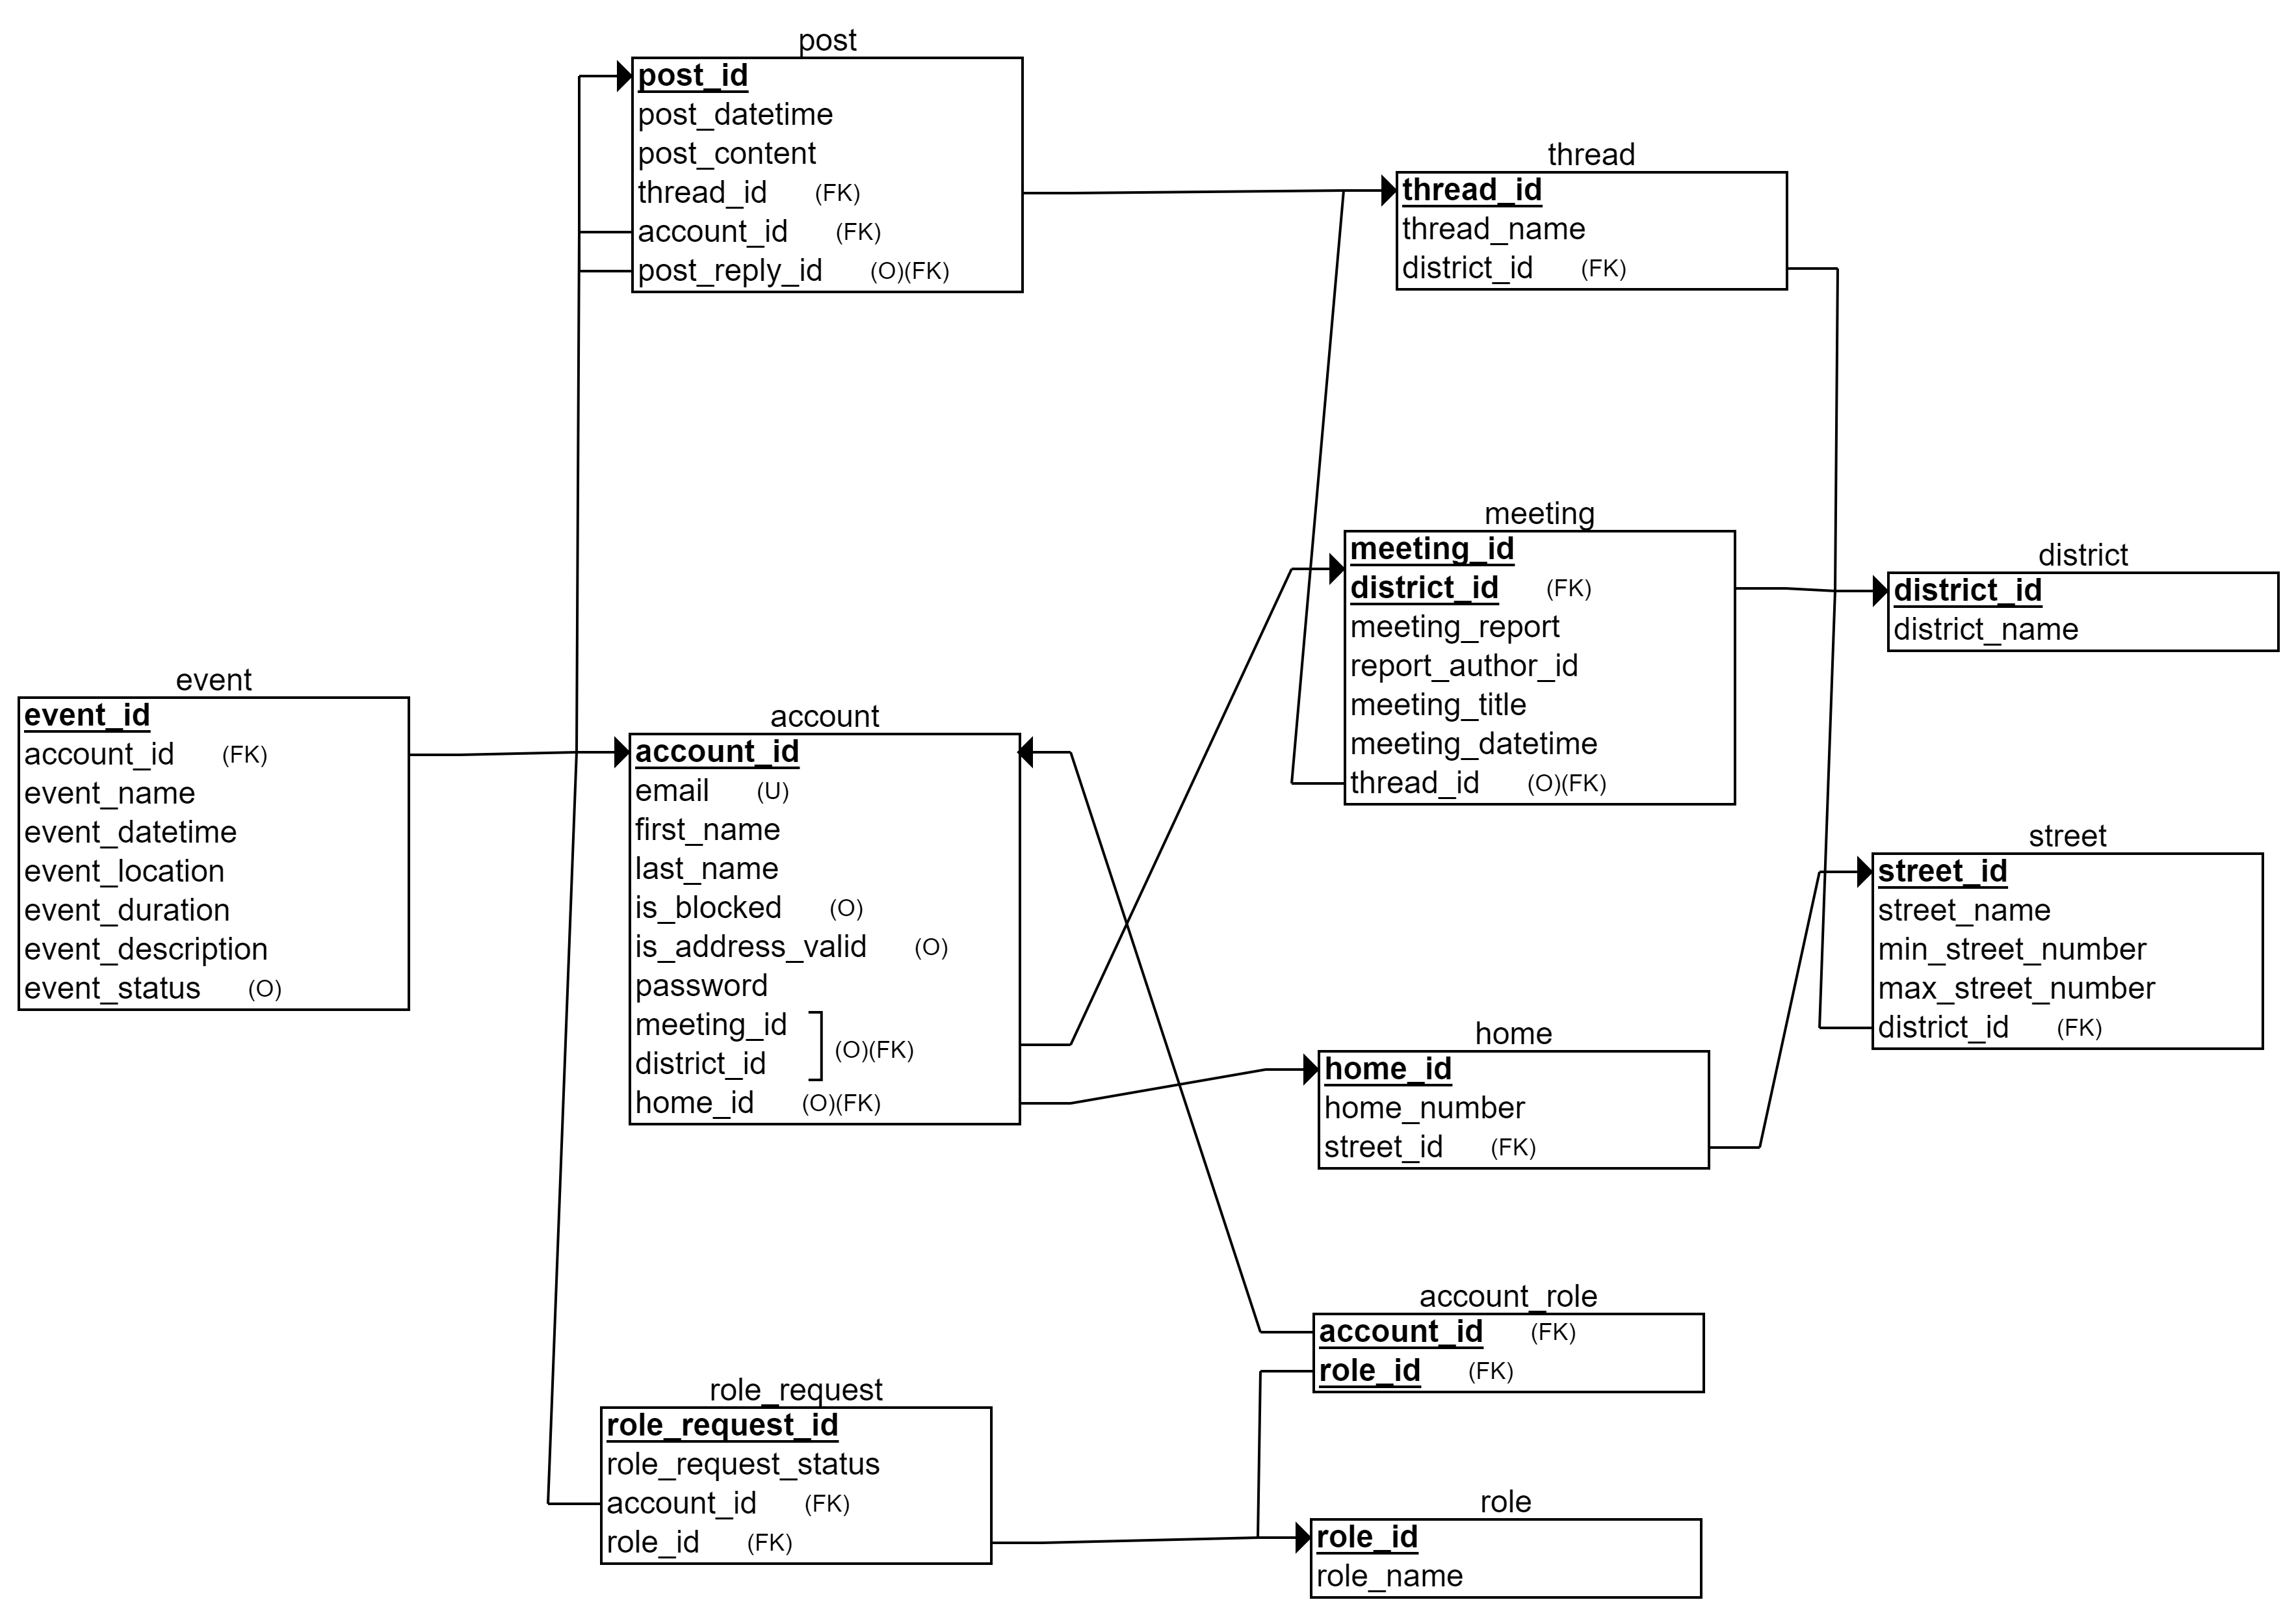
\includegraphics[width = 200mm,scale = 3]{11 relacijska shema baze podataka.png}}
  \caption{Relacijska shema baze podataka}
  \label{Relacijska_shema}
\end{figure}
			
			\eject
			
		\section{Dijagram razreda}
		
		Backend aplikacije je ostvaren korištenjem radnog okvira Spring Boot, i stoga aplikacija ima nekoliko slojeva.
		
		Iako se ne smatraju posebnim slojem, na slici 4.2 prikazani su entiteti koji odgovaraju relacijama u bazi podataka, opisanoj u poglavlju 4.1. Entiteti ne sadrže nikakvu proceduralnu logiku, nego isključivo članske varijable i njihove gettere i settere. Entitetu našoj aplikaciji su redom: Account, District, Event, Home, Meeting, Post, Role, RoleRequest, Street i PostThread.
		
		Na slici 4.3 prikazan je sloj Repository. Razredi u njemu se definiraju kao sučelja koja nude metode dohvaćanja elemenata iz baze, te stvaranja promjena u bazi. Njihov kod u pravilu programer ne piše eksplicitno, nego te metode generira Spring na temelju njihovog imena.
		
		Na slici 4.4 prikazan je sloj Service. Taj sloj sadrži centralnu logiku na backendu, manipulira entitetima i poziva metode koje nudi prethodni sloj, Repository.
		
		Na slici 4.5 prikazan je sloj Controller. Taj je sloj najviši u hijerarhiji slojeva, i on je jedini sloj s kojim komunicira frontend dio aplikacije. Uloga ovog sloja je da obrađuje HTTP zahtjeve, poziva metode koje nudi prethodni sloj Service, i potom odgovara na primljene zahtjeve.
		
		Zbog preglednosti, na jednom dijagramu nije bilo moguće prikazati sve razrede. Umjesto toga, na sljedeći način su prikazani odnosi među slojevima: na slici 4.6 prikazan je odnos između slojeva Controller i Service, na slici 4.7 prikazan je odnos između slojeva Service i Repository, na slici 4.8 prikazan je odnos između sloja Service i entiteta, te je na slici 4.9 prikazan odnos između sloja Repository i entiteta.
		
		\eject
		
				\begin{figure}[H]
					\centering
					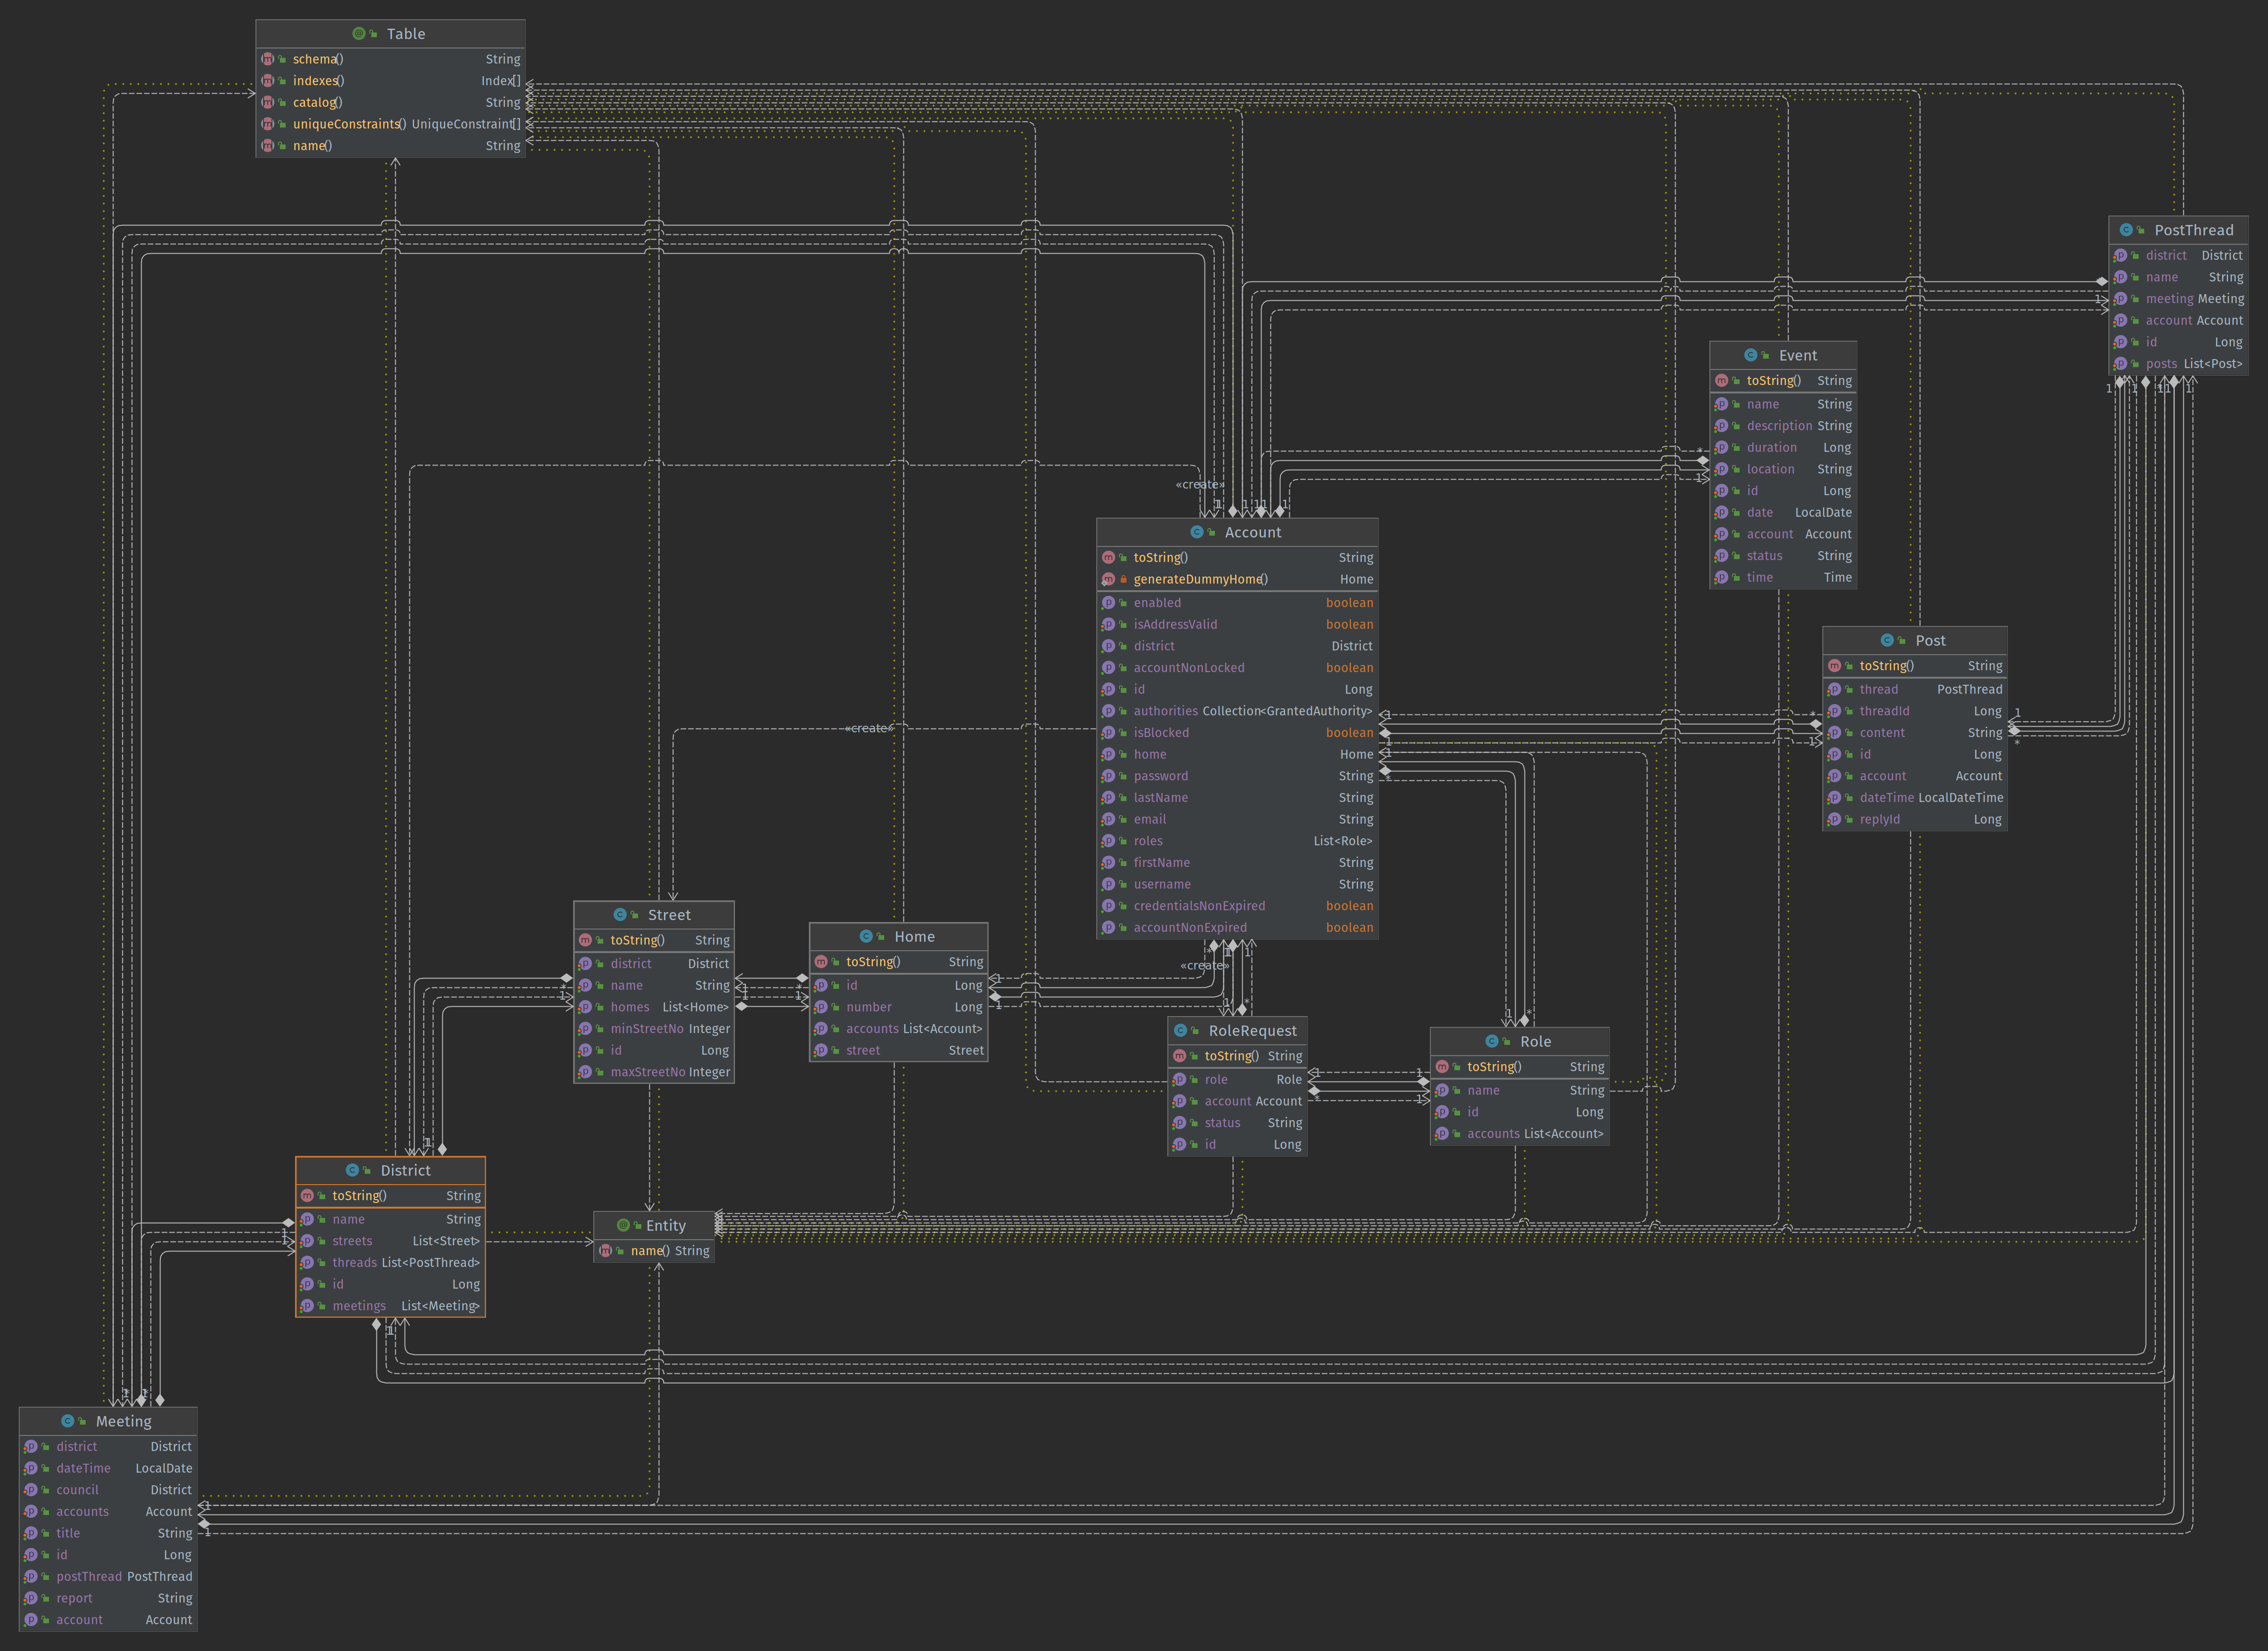
\includegraphics[width=\textwidth,keepaspectratio]{12.1 entiteti.png}
					\caption{Dijagram razreda - entiteti}
				\end{figure}	
				
				\begin{figure}[H]
					\centering
					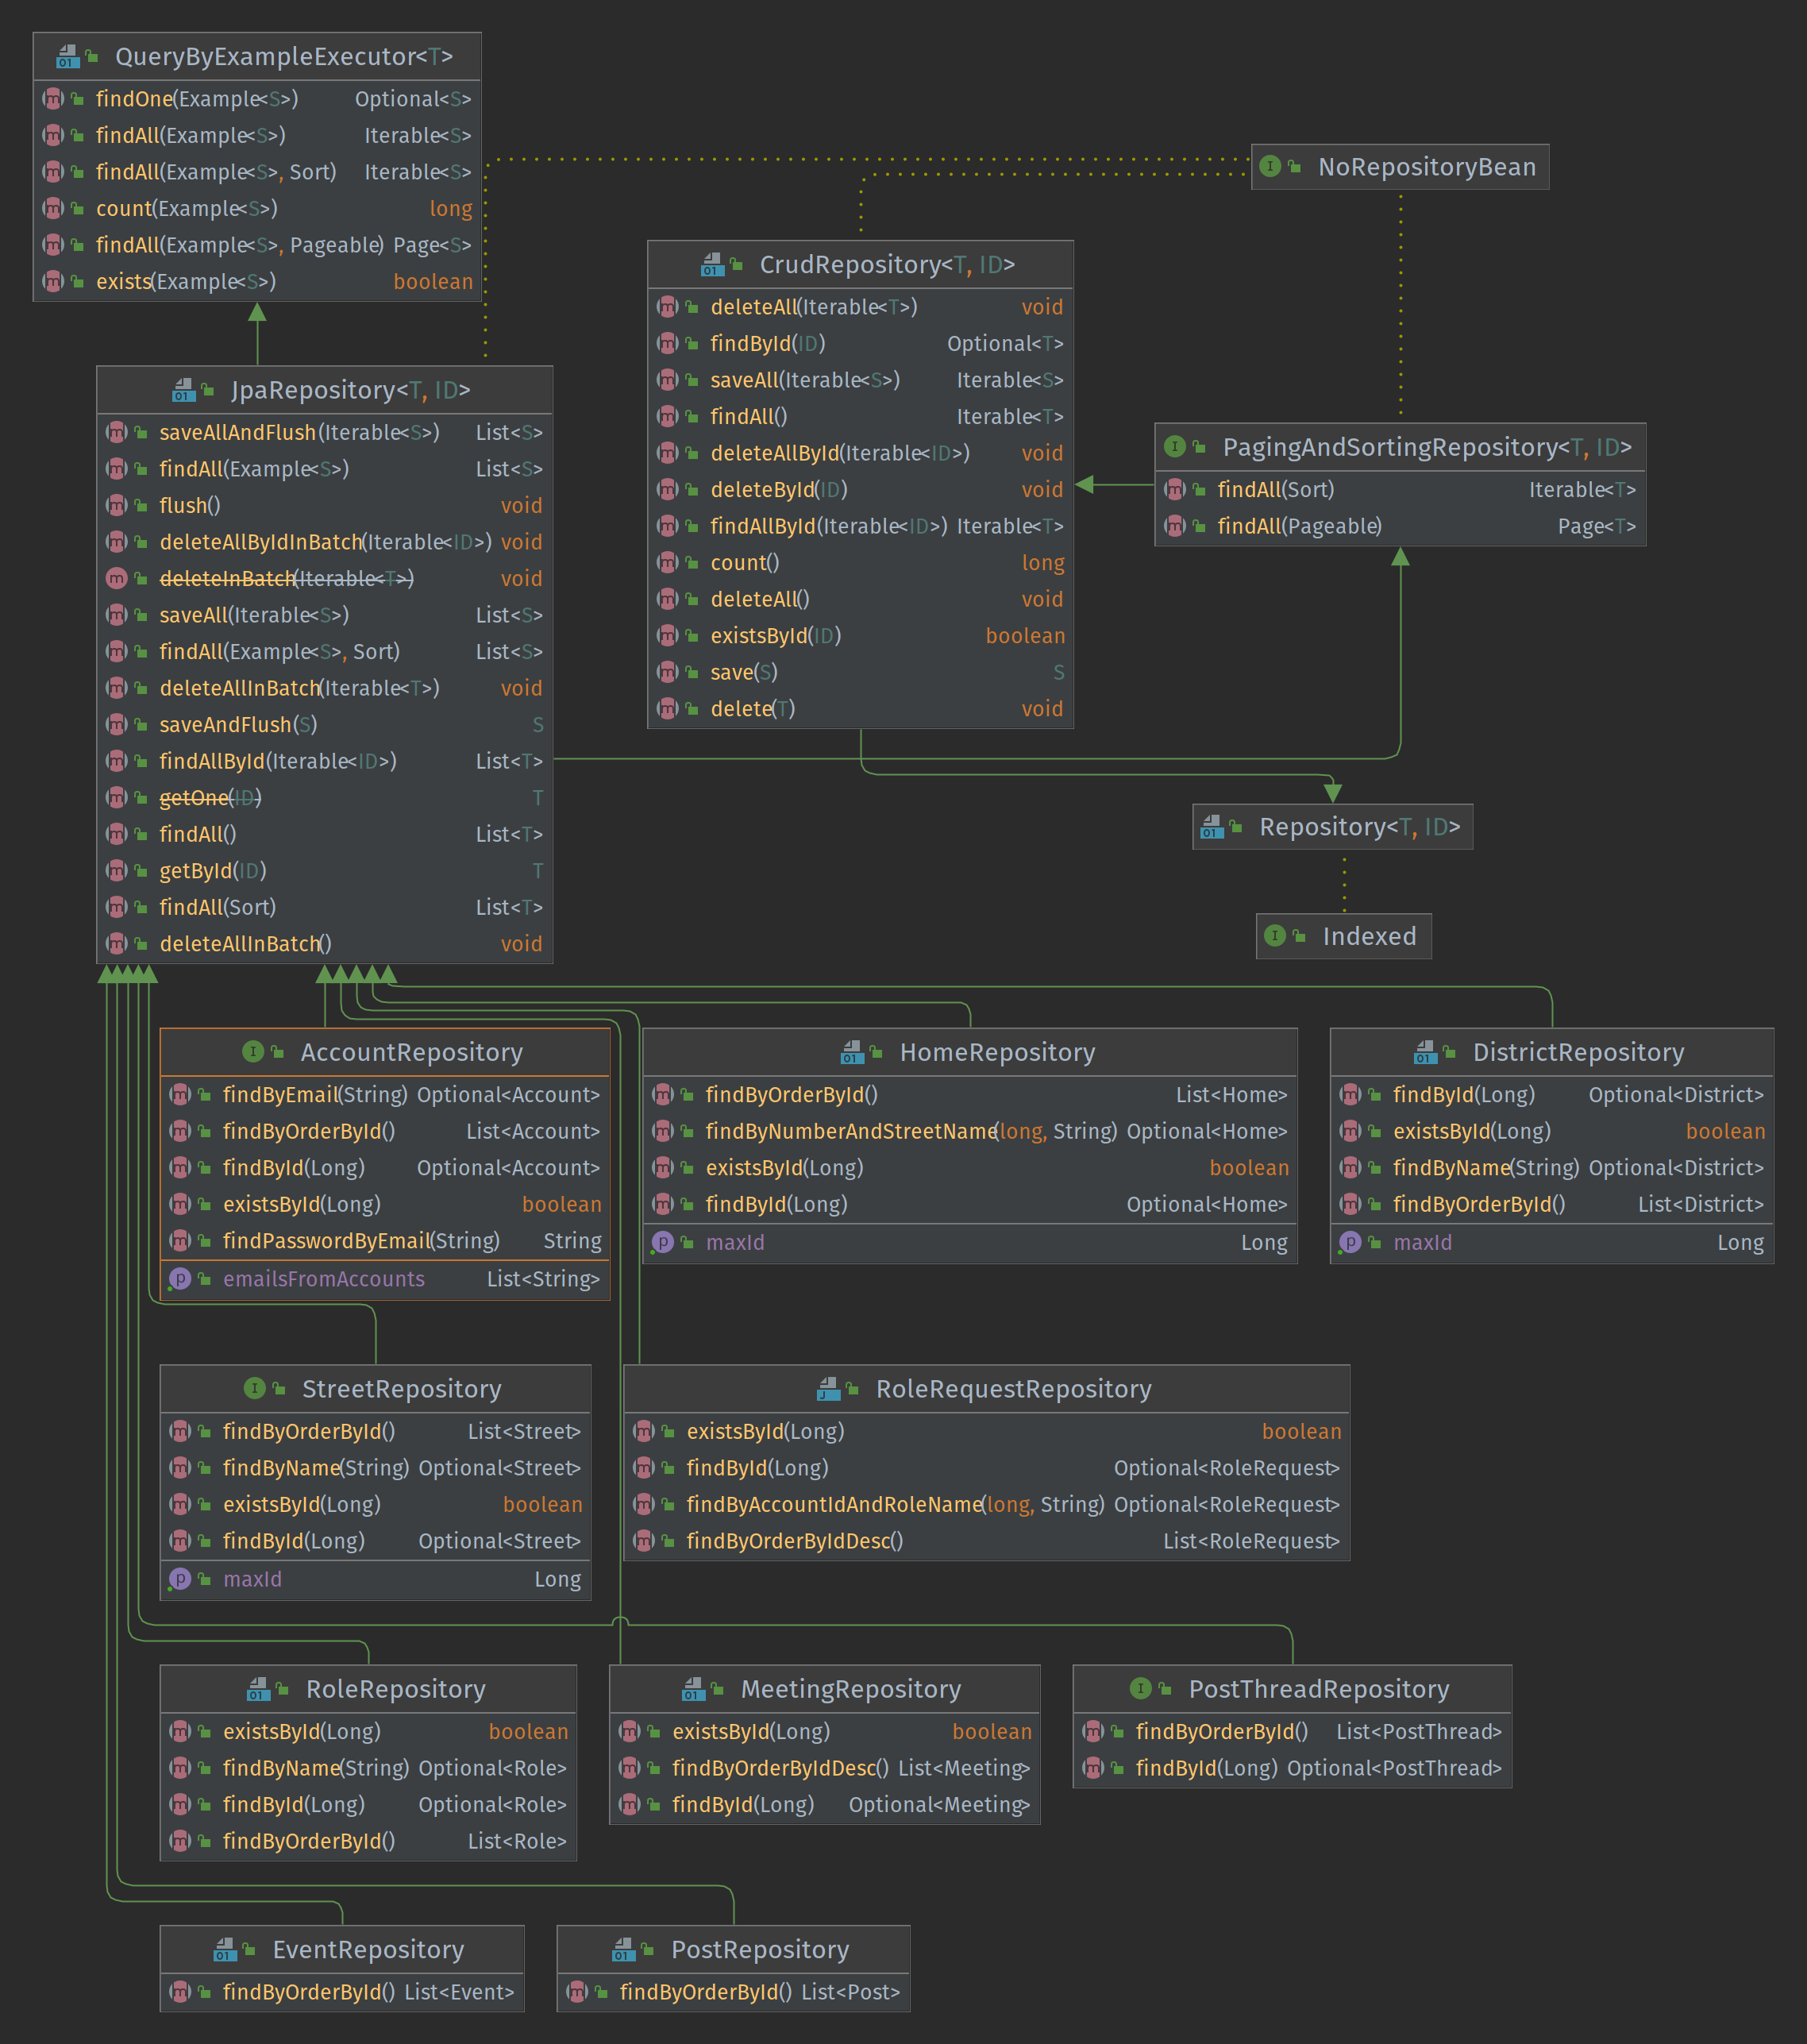
\includegraphics[width=\textwidth,keepaspectratio]{12.2 repozitoriji.png}
					\caption{Dijagram razreda - sloj Repository}
				\end{figure}	
				
				\begin{figure}[H]
					\centering
					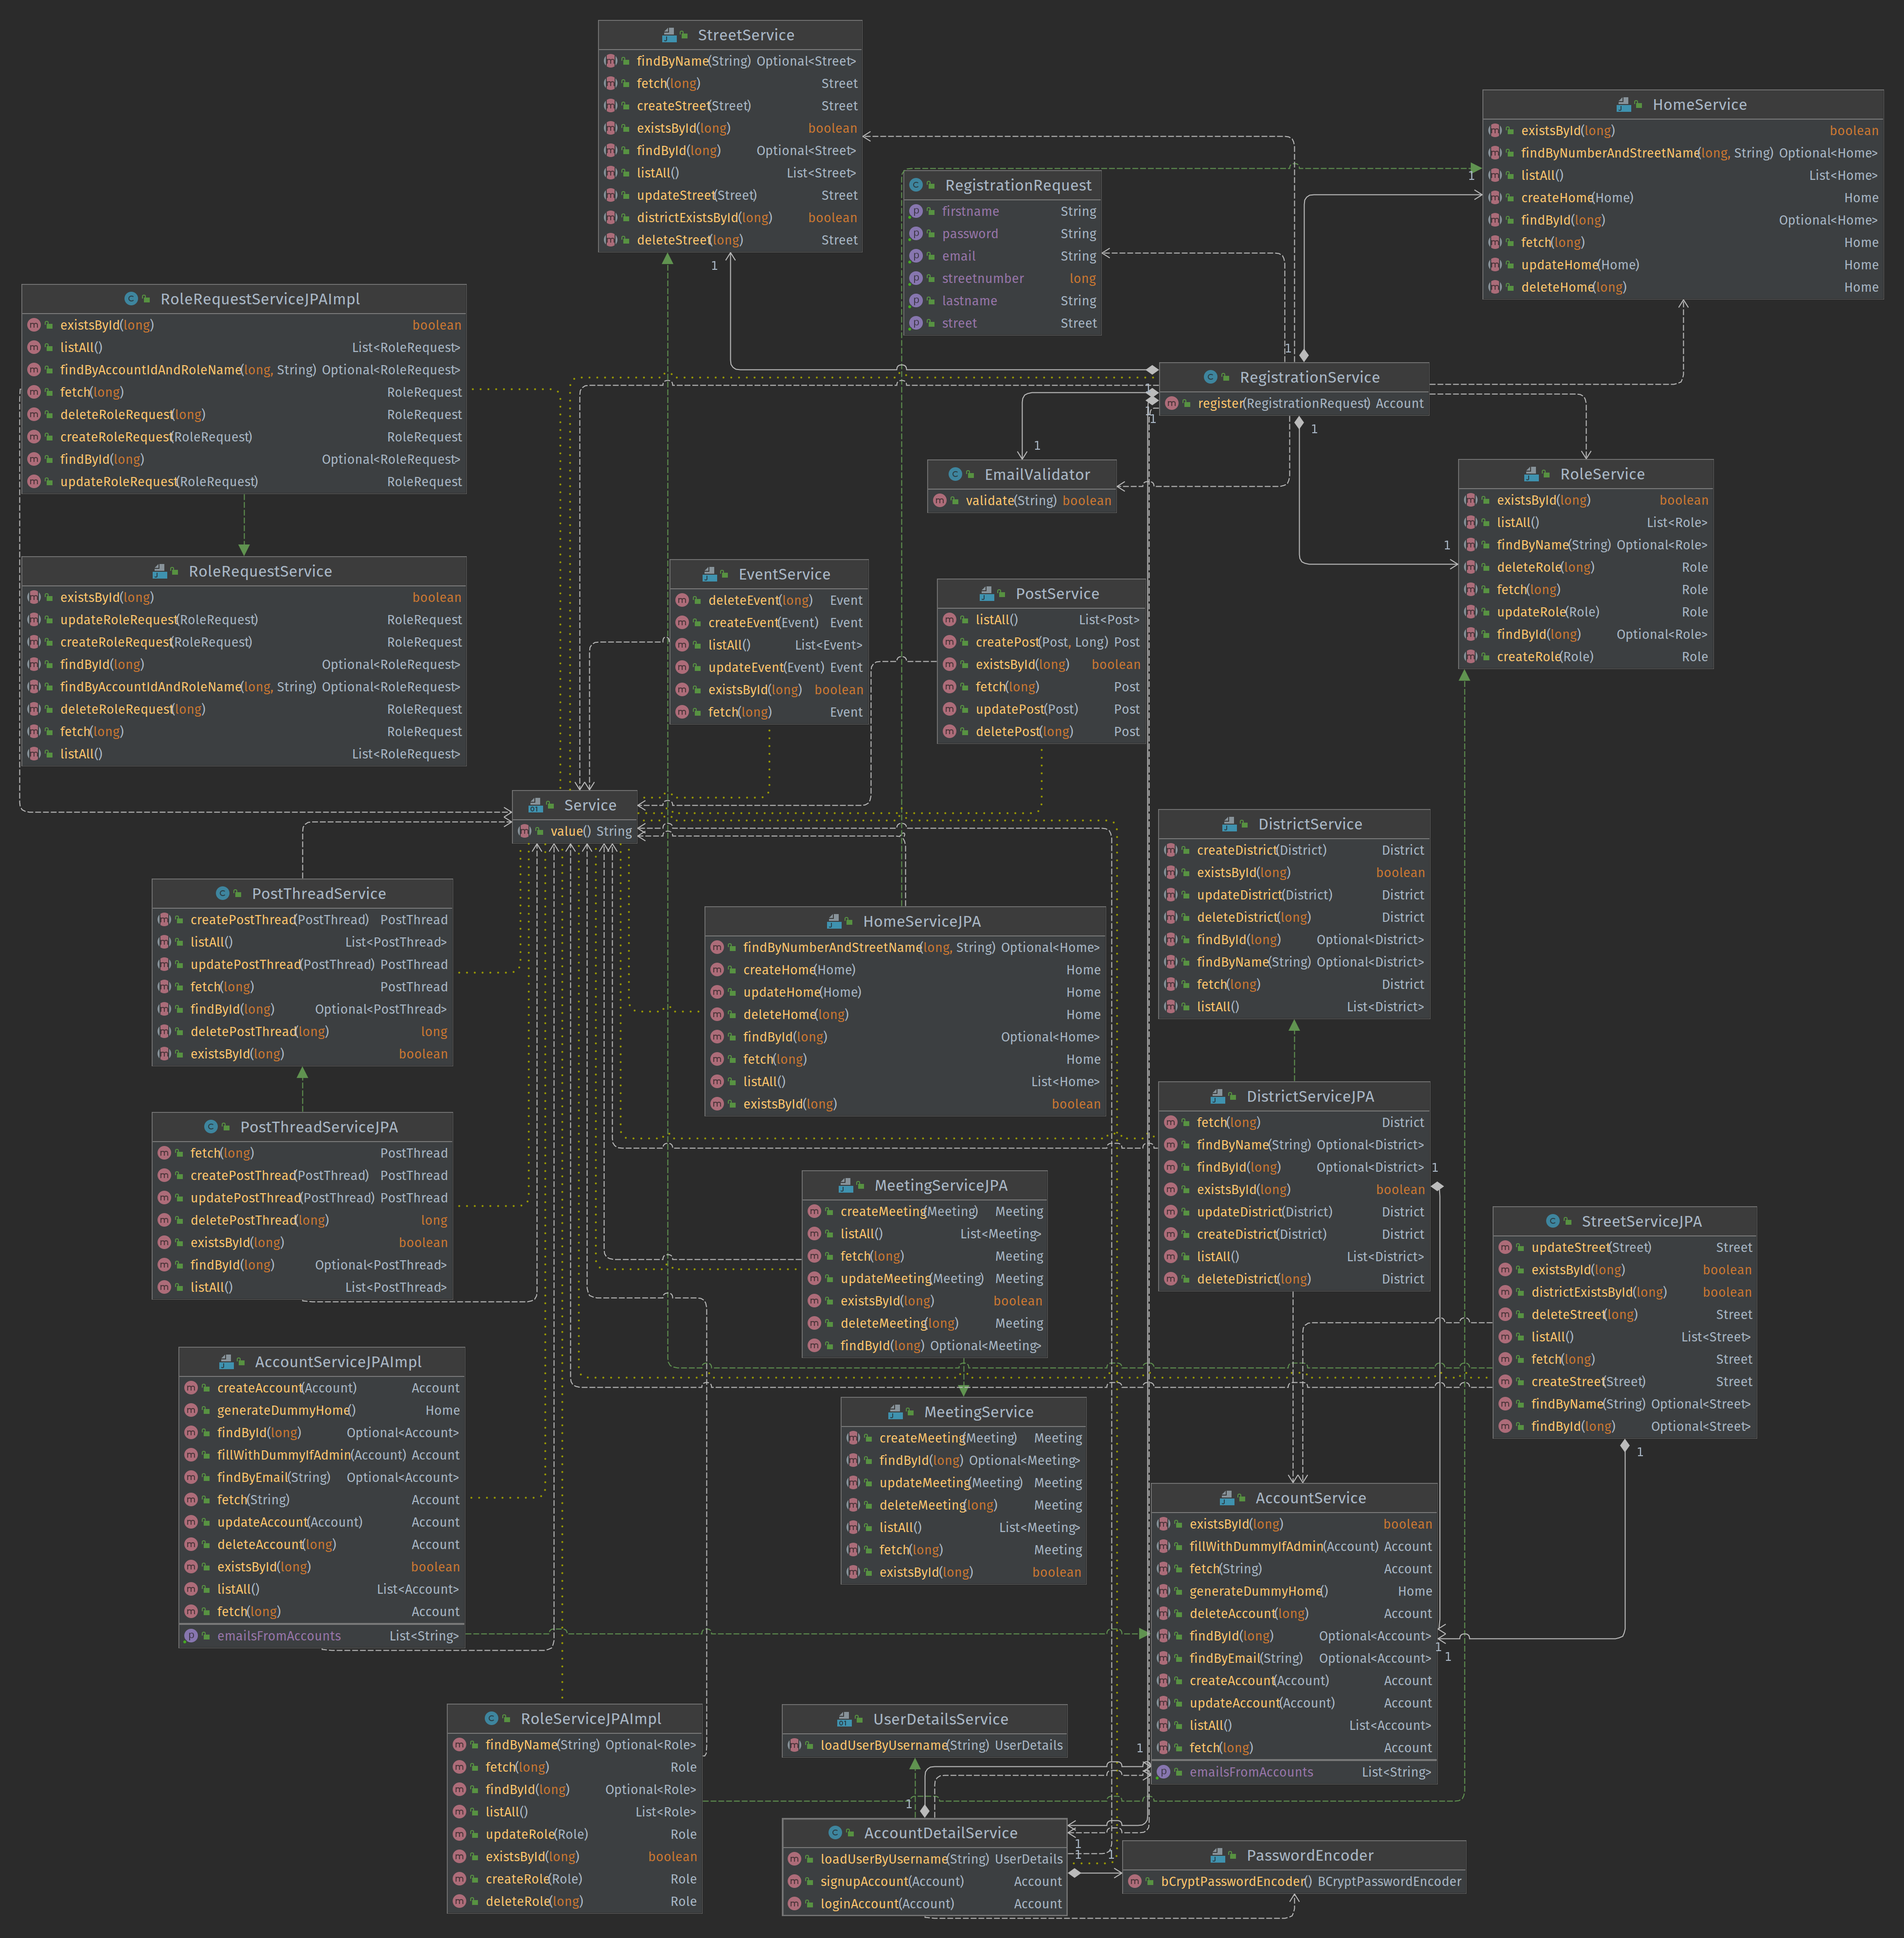
\includegraphics[width=\textwidth,keepaspectratio]{12.3 servisi.png}
					\caption{Dijagram razreda - sloj Service}
				\end{figure}	
				
				\begin{figure}[H]
					\centering
					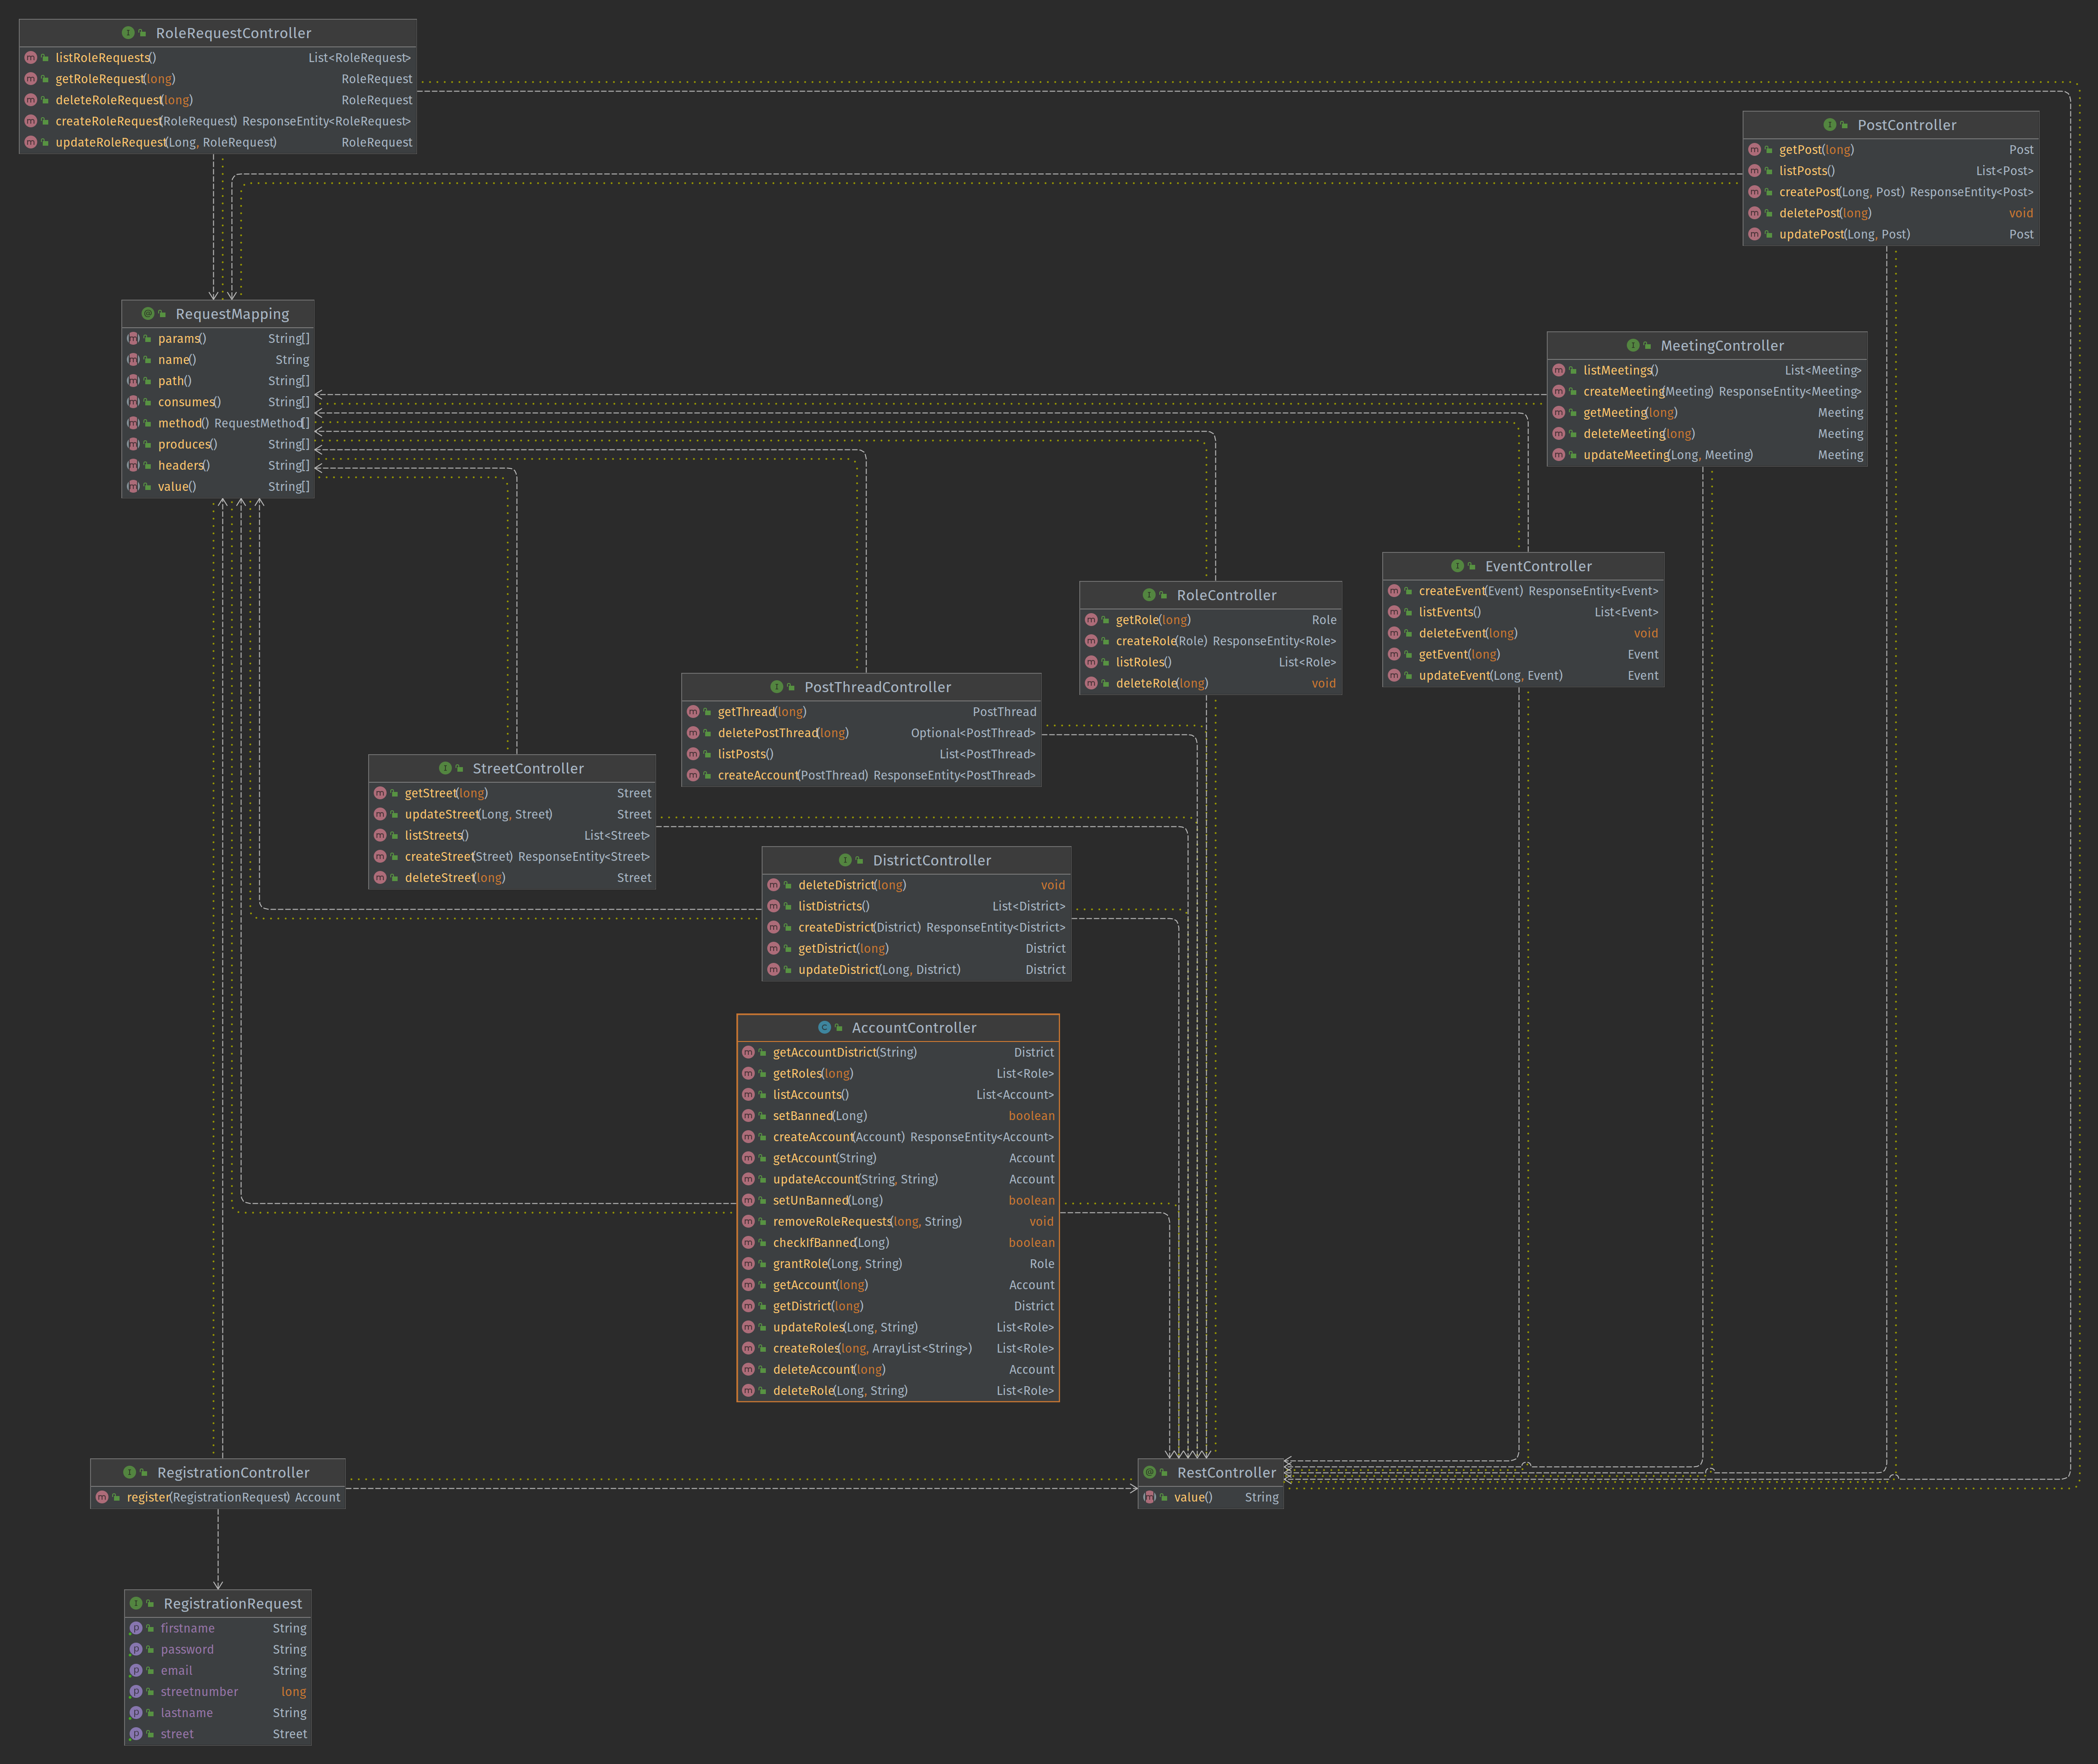
\includegraphics[width=\textwidth,keepaspectratio]{12.4 kontroleri.png}
					\caption{Dijagram razreda - sloj Controller}
				\end{figure}	
				
				\begin{figure}[H]
					\centering
					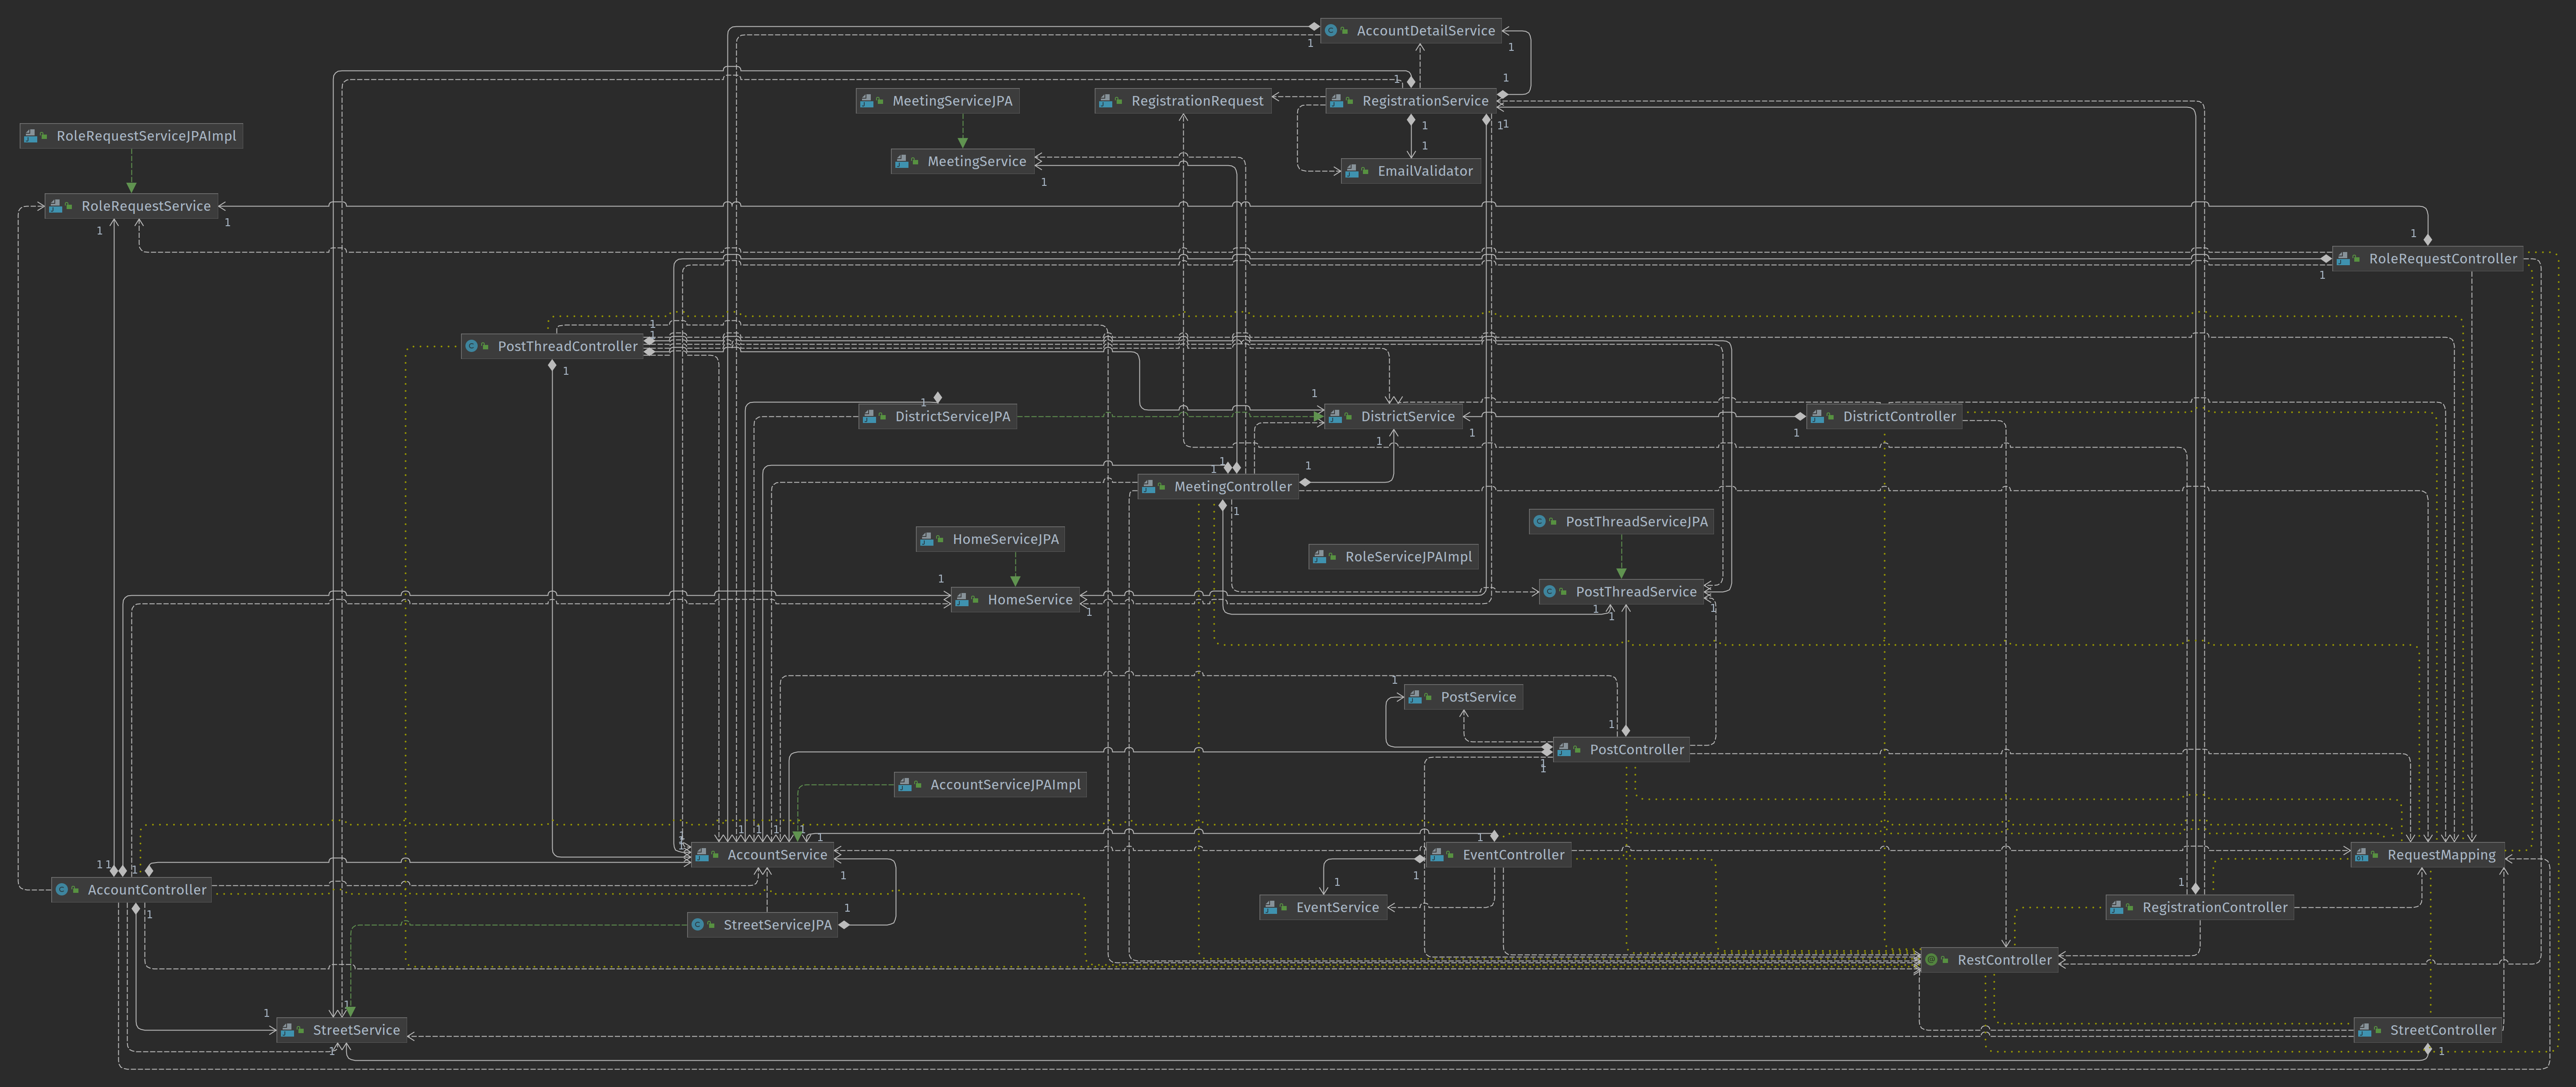
\includegraphics[width=\textwidth,keepaspectratio]{13.1 kontroleri i servisi.png}
					\caption{Dijagram razreda - odnos slojeva Controller i Service}
				\end{figure}	
				
				\begin{figure}[H]
					\centering
					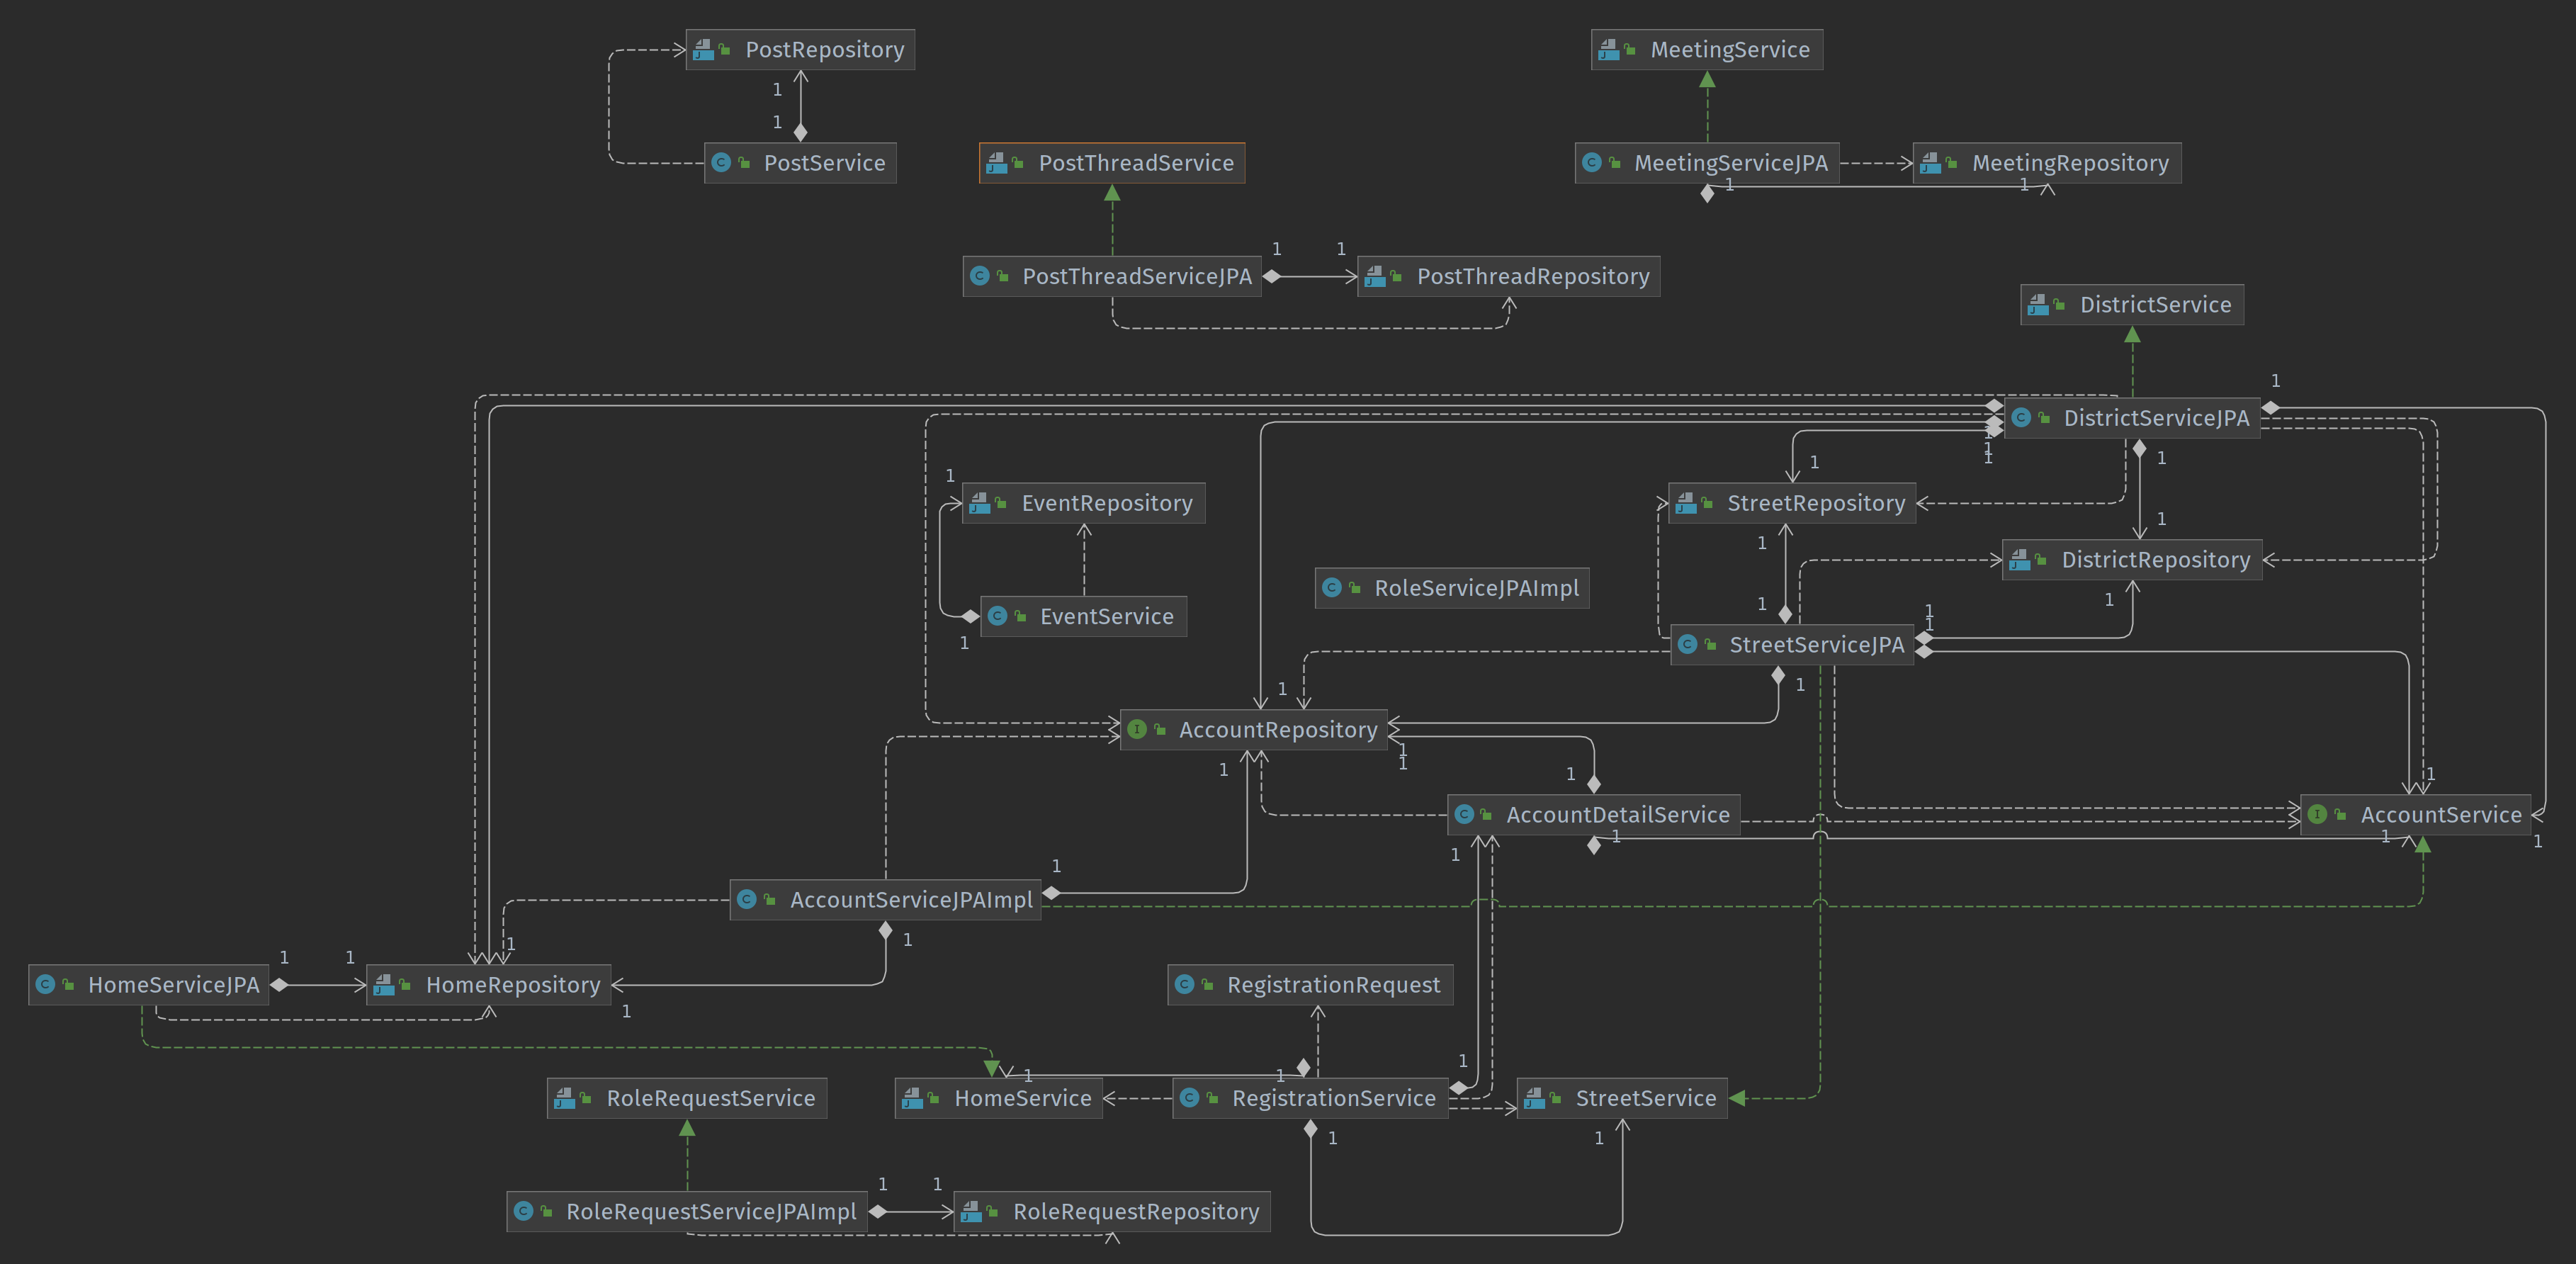
\includegraphics[width=\textwidth,keepaspectratio]{13.2 servisi i repozitoriji.png}
					\caption{Dijagram razreda - odnos slojeva Service i Repository}
				\end{figure}	
				
				\begin{figure}[H]
					\centering
					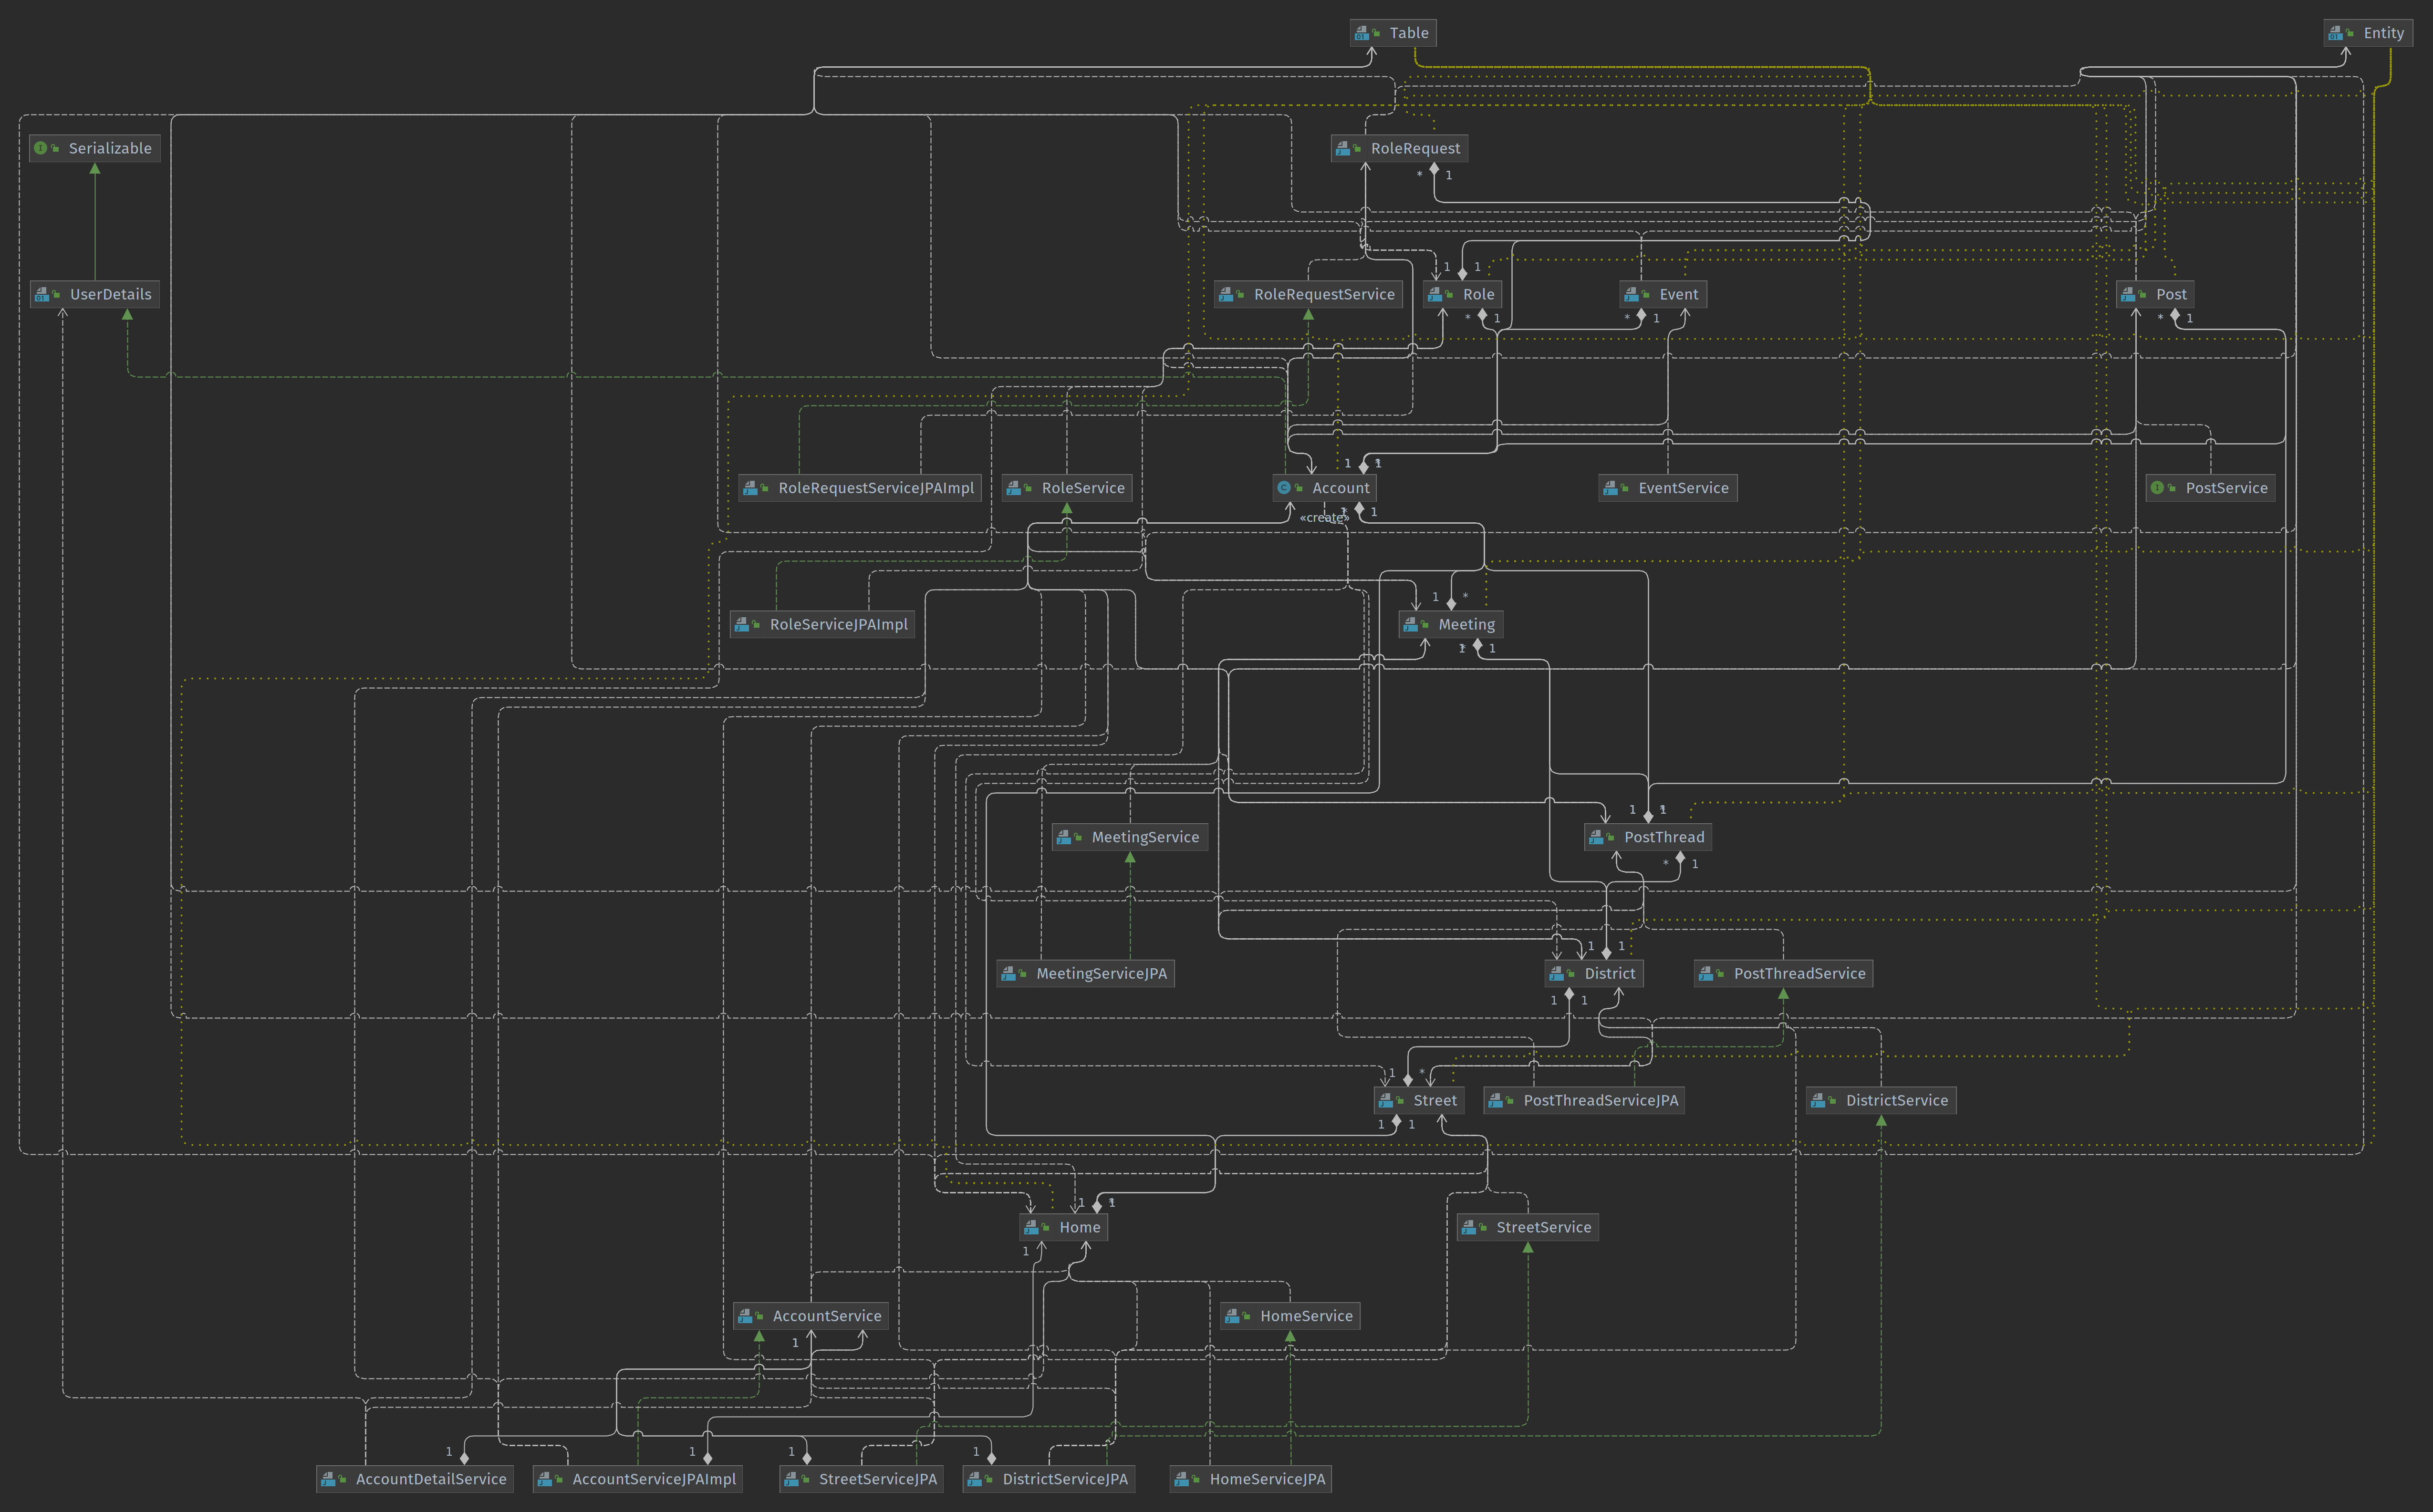
\includegraphics[width=\textwidth,keepaspectratio]{13.3 servisi i entiteti.png}
					\caption{Dijagram razreda - odnos sloja Service i entiteta}
				\end{figure}	
				
				\begin{figure}[H]
					\centering
					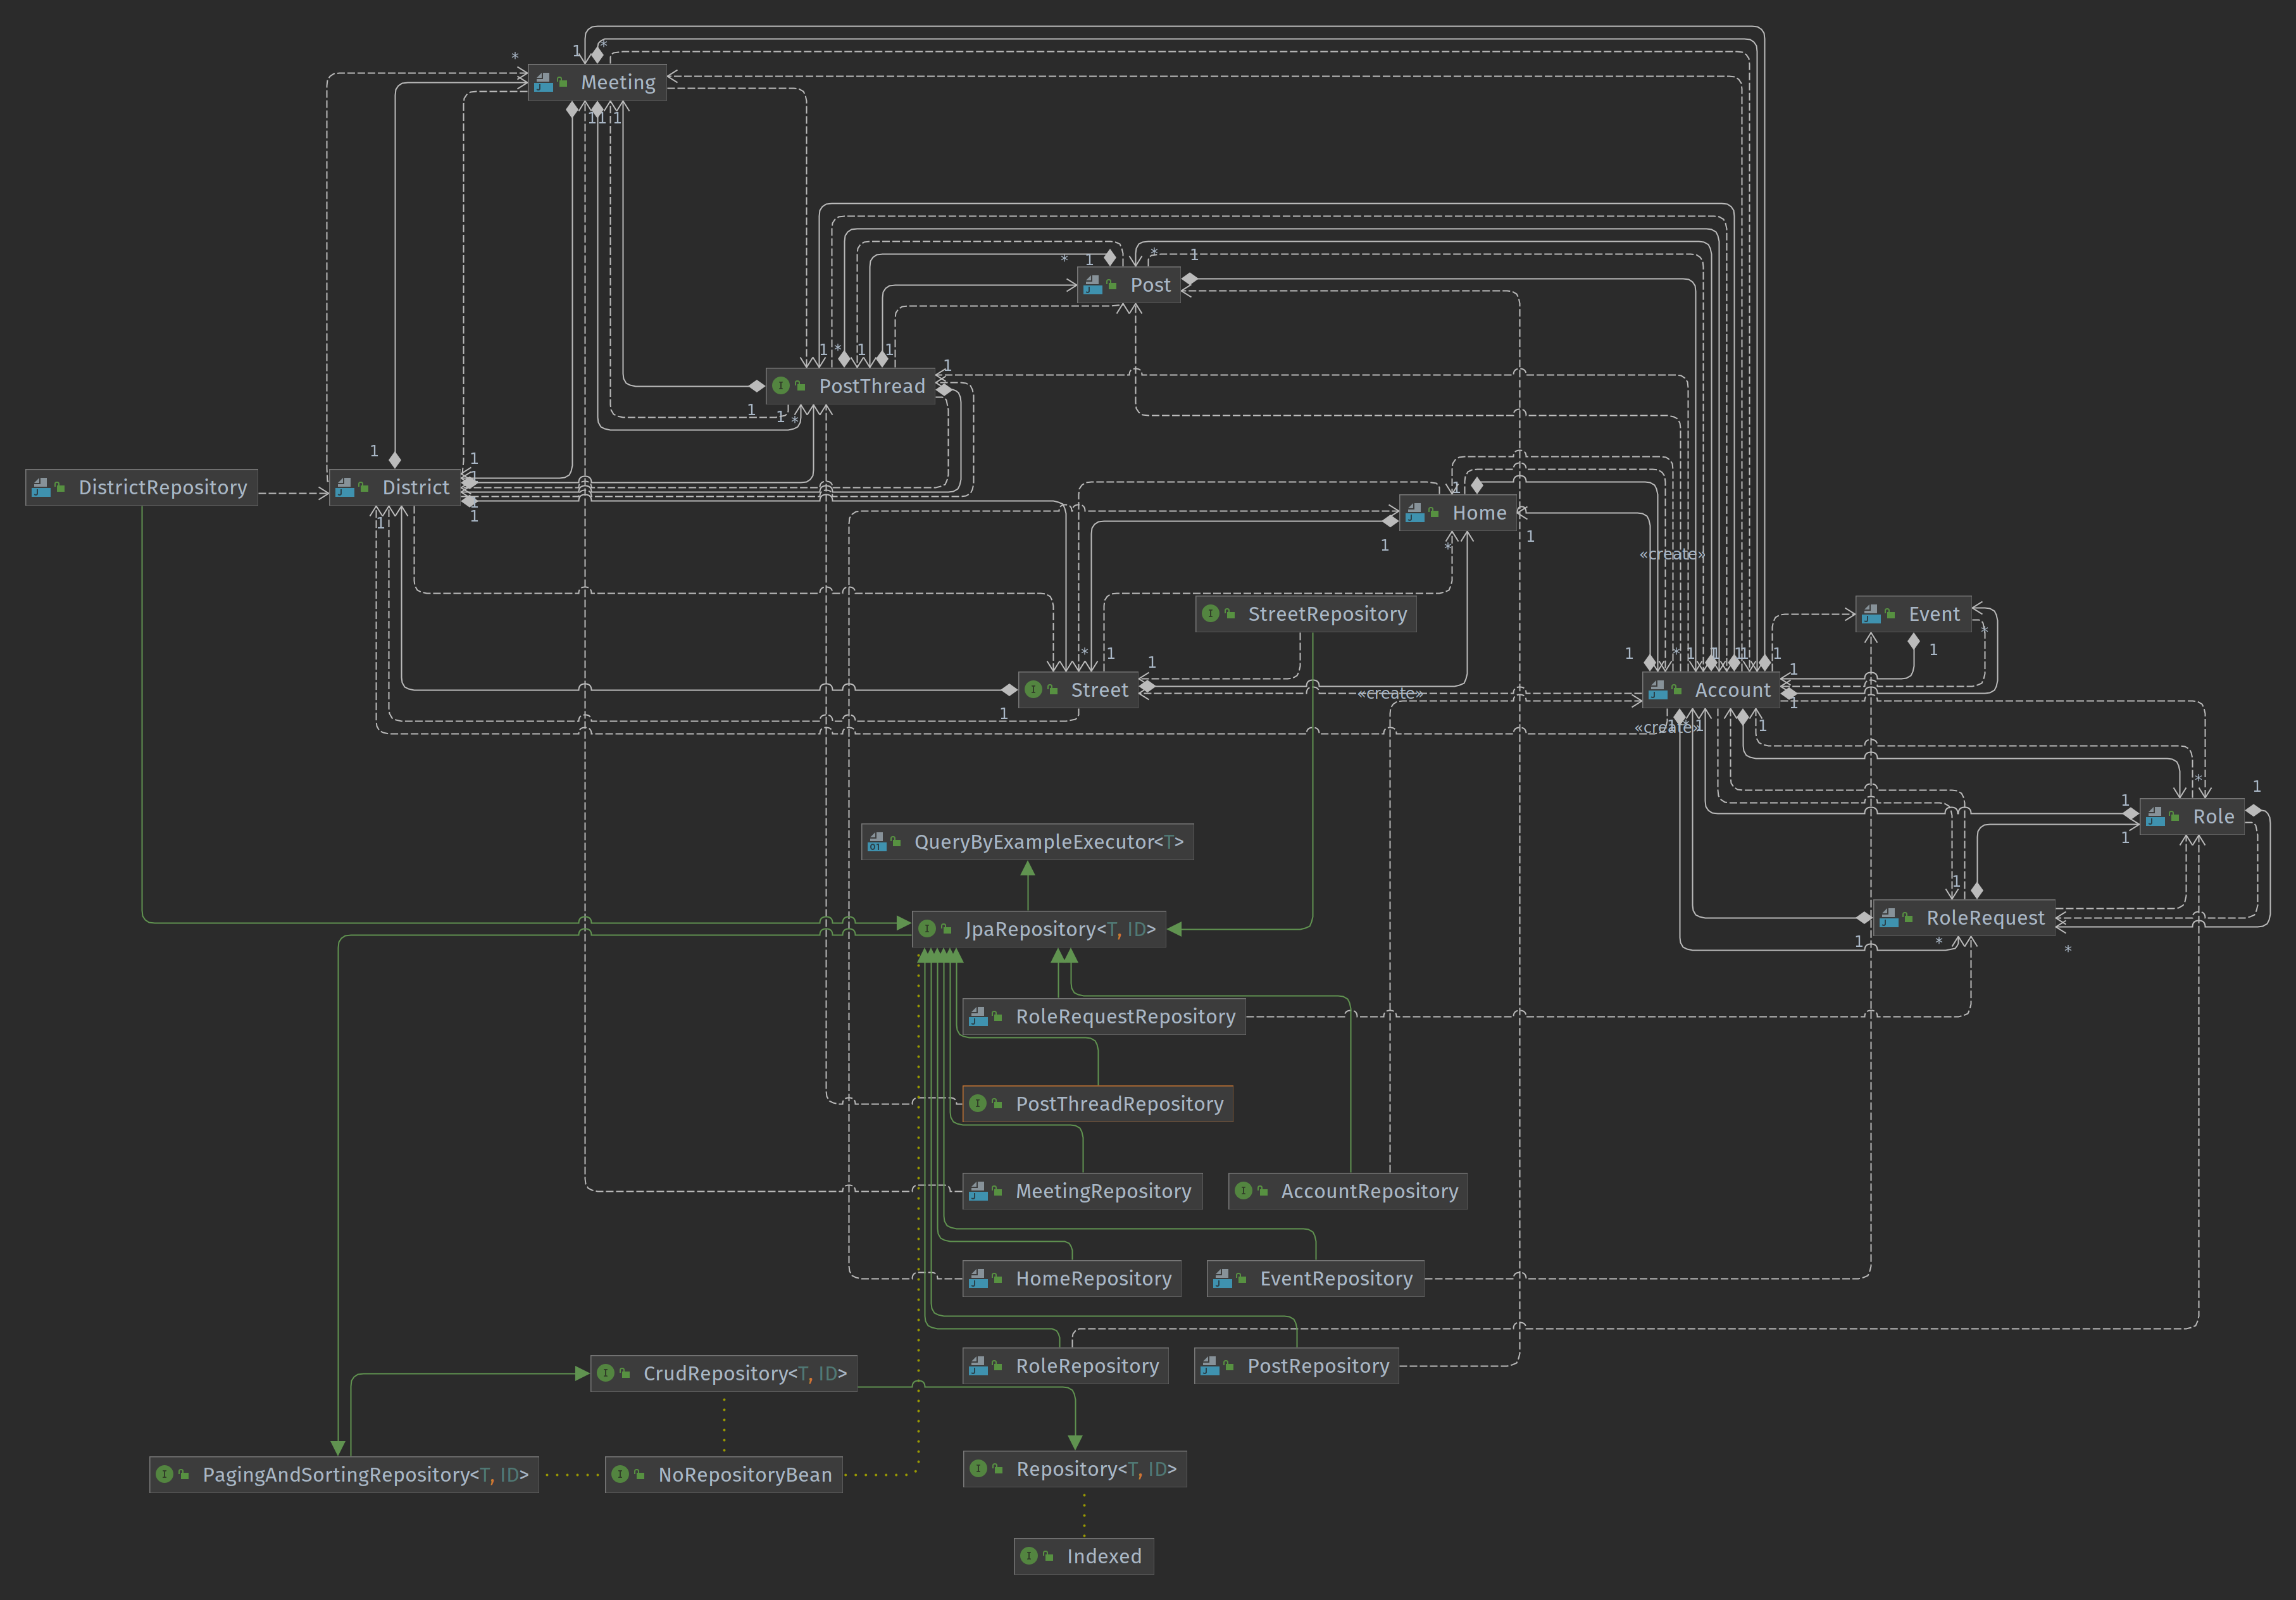
\includegraphics[width=\textwidth,keepaspectratio]{13.4 repozitoriji i entiteti.png}
					\caption{Dijagram razreda - odnos sloja Repository i entiteta}
				\end{figure}	
			
			
			\eject
			
		
		\section{Dijagram stanja}
		
		Na slici 4.10 prikazan je dijagram stanja korisničkog sučelja. Stranica na koju korisnik uvijek prvo dođe je "Prijava". S te stranice korisnik može birati opciju "Registracija" kako bi stvorio novi račun, ili se može prijaviti s postojećim računom. Ovisno o tome je li korisnik stanovnik ili administrator, dočeka ga prikladna početna stranica. 
		
		Ako je korisnik stanovnik, sa svoje početne stranice može birati opcije "Osobni podaci", "Događaji", "Vijeće četvrti" i "Forum". Pri pregledu svojih osobnih podataka, korisnik može slati zahtjeve za dodatne uloge ili mijenjati svoje osobne podatke. Pri pregledu sekcije "Događaji", korisnik može stvarati prijedloge događaja. Pri pregledu sekcije "Vijeće četvrti", korisnik klikom na pojedino izvješće može dobiti dodatne informacije o tom izvješću, a ako ima ulogu "Vijećnik", onda može i stvarati nova izvješća. Konačno, pregledom sekcije "Forum" korisnik može otvarati nove teme i pregledavati postojeće.
		
		Ako je korisnik administrator, sa svoje početne stranice može birati opcije "Osobni podaci", "Zahtjevi za uloge", "Korisnici" i "Kvartovi". Prilikom pregleda svojih osobnih podataka, administrator može neke od tih podataka može mijenjati. Prilikom pregleda zahtjeva za uloge administrator može odabrati pojedini zahtjev te ga prihvatiti ili odbiti. Prilikom pregleda svih korisnika sustava, administrator može odabrati pojedinog korisnika i dobiti više informacija o njemu. Konačno, pri pregledu kvartova, administrator može dodati novi kvart, a može i za postojeći kvart odabrati opciju unosa nove ulice.
		
		Iako zbog preglednosti to nije navedeno na dijagramu, stanovnici iz svih stanja mogu doći u stanja "Početna stranica", "Događaji", "Vijeće četvrti", "Forum" i "Osobni podaci", te administratori analogno mogu iz svih stanja doći u stanja "Početna stranica", "Korisnici", "Kvartovi", "Zahtjevi uloga" i "Osobni podaci". Također, svi korisnici iz svih stanja mogu birati opciju "Odjava" i preći u stanje "Prijava".
			
			
						\begin{figure}[H]
					\centering
					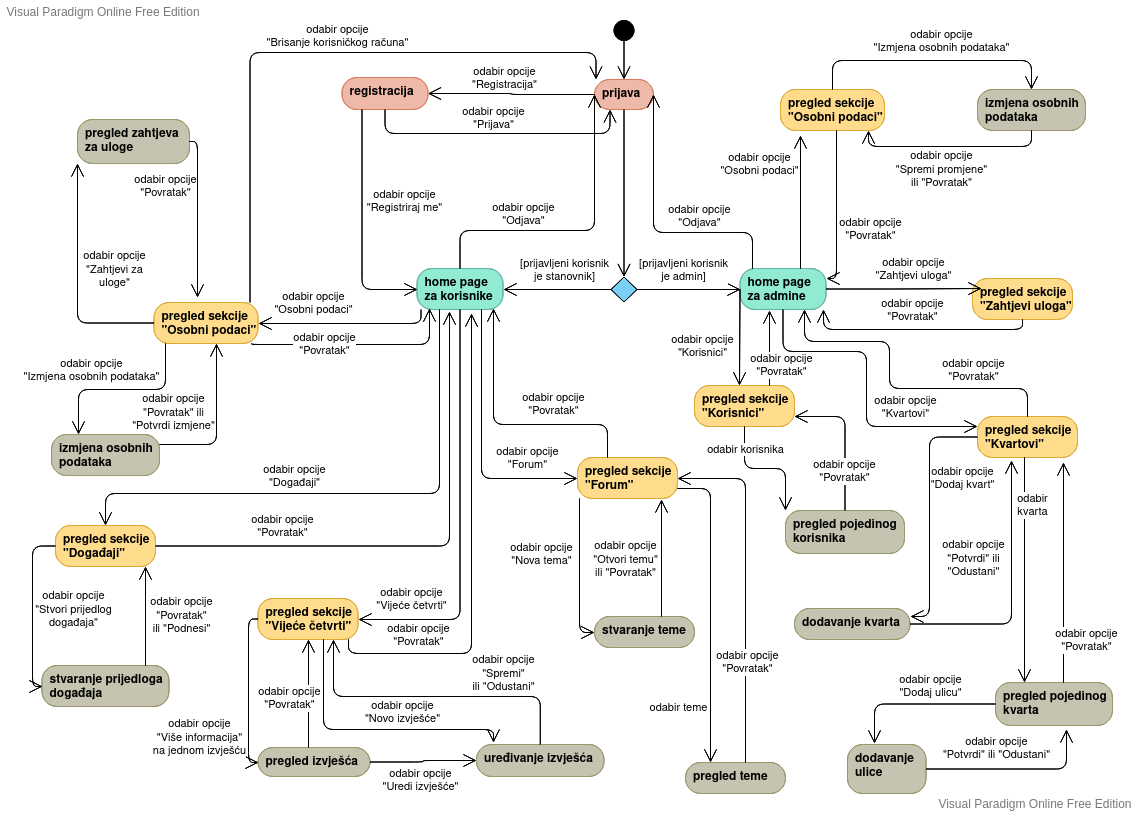
\includegraphics[width=\textwidth,keepaspectratio]{14 dijagram stanja.png}
					\caption{Dijagram stanja}
				\end{figure}	
			
			
			\eject 
		
		\section{Dijagram aktivnosti}
		
		Na slici 4.11 prikazan je dijagram aktivnosti prilikom stvaranja novih događaja. Korisnik koji želi predložiti događaj ispunjava formu u koju unosi naziv, mjesto, vrijeme, trajanje i kratki opis. Kada ju je ispunio, odabire opciju spremanja prijedloga. Web aplikacija tada provjerava jesu li svi traženi podaci u ispravnom formatu. Ako nisu, upozorava korisnika na pogreške i omogućuje mu da ih ispravi, a ako su podaci ispravni, onda sprema prijedlog u bazu podataka. Nakon što je prijedlog spremljen, moderator ga može pregledati. Ako moderator procijeni da prijedlog ne zadovoljava jezični standard, može ga uređivati. Kada je ispravio sve eventualne pogreške, moderator odabire opciju spremanja promjena. Tada web aplikacija provjerava jesu li svi podaci u ispravnom formatu, te ako jesu, sprema promjene, a ako nisu, upozorava moderatora na pogreške i omogućuje mu da ih ispravi. Nakon što je završio s eventualnim uređivanjem prijedloga, moderator može odabrati opciju prihvaćanja ili odbijanja prijedloga, i u oba slučaja se ažurira status prijedloga događaja u bazi podataka.
			
			\begin{figure}[H]
					\centering
					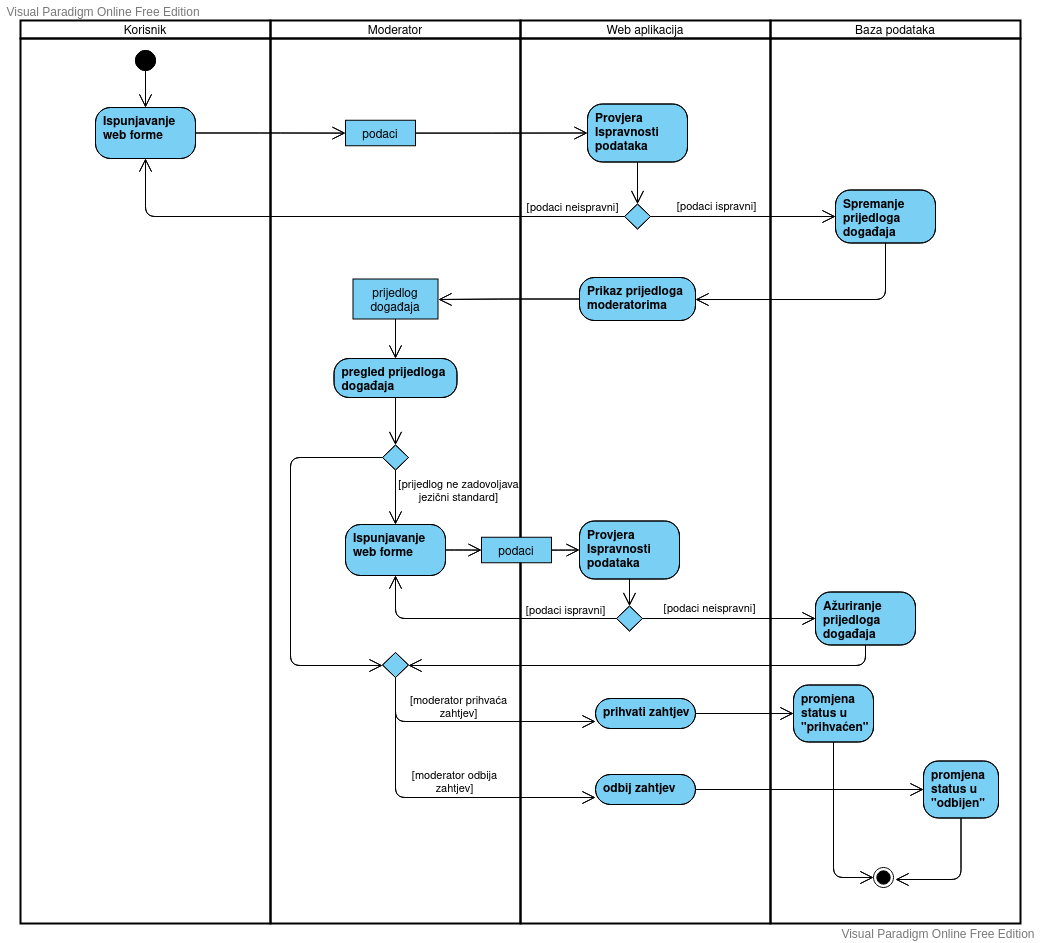
\includegraphics[width=\textwidth,keepaspectratio]{15 dijagram aktivnosti.png}
					\caption{Dijagram aktivnosti}
				\end{figure}	
			
			\eject
		\section{Dijagram komponenti}
		
		 Na slici 4.12 prikazan je dijagram komponenti. Korisnik iz web preglednika pristupa pristupa aplikaciji korištenjem REST API-ja. Sama aplikacija se sastoji od dvije komponente. Prva komponenta odgovara frontendu i izgrađena je korištenjem React biblioteke. Druga komponenta odgovara backendu i izgrađena je korištenjem radnog okvira Spring. Frontend i backend komuniciraju korištenjem REST API-ja. Baza podataka je relacijska i backend joj pristupa slanjem SQL upita.
		
			\begin{figure}[H]
					\centering
					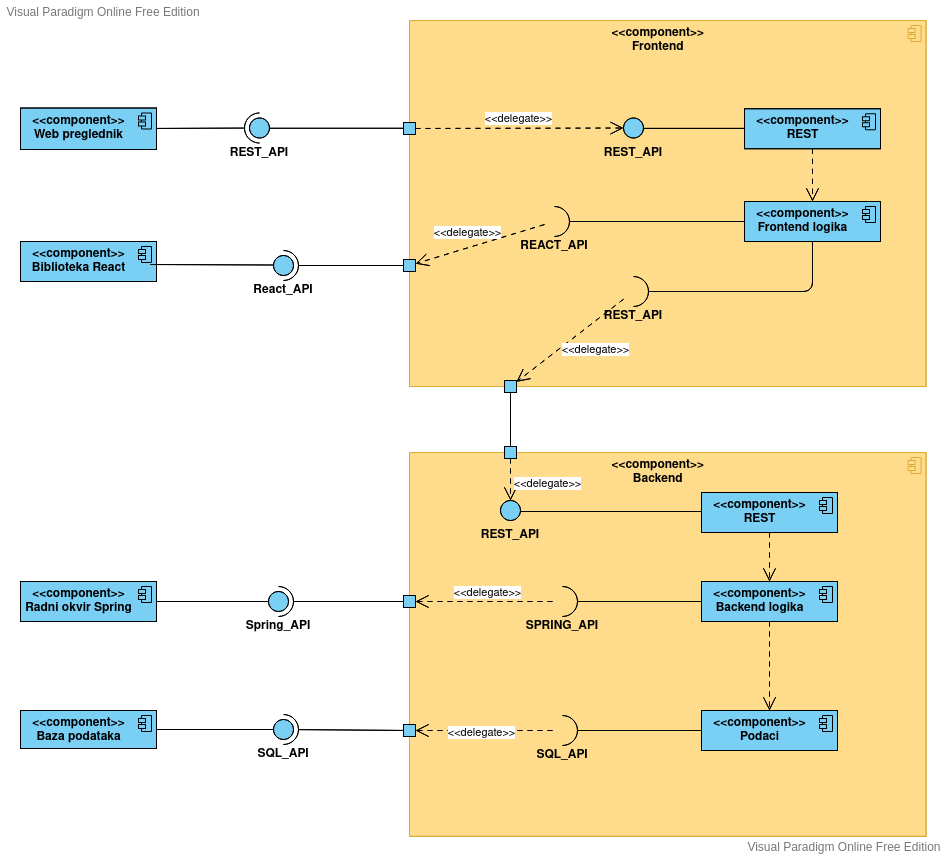
\includegraphics[width=\textwidth,keepaspectratio]{16 dijagram komponenti.png}
					\caption{Dijagram komponenti}
				\end{figure}	
				\newpage			
